% !TeX program = lualatex
% !BIB program = biber
% !TeX encoding = UTF-8
%
% ============================================================
% TRABAJO FINAL DE DIPLOMADO - MONOGRAFÍA
% UNIVERSIDAD AUTÓNOMA JUAN MISAEL SARACHO
%
% DIPLOMADO EN DESARROLLO WEB Y APLICACIONES MÓVILES
%
% POSTULANTE:
% Adrian Alejandro Llanos Zenteno
%
% PROYECTO:
% Sistema web y móvil de gestión de pacientes y radiografías
% dentales para la Clínica Odontológica San Martín
%
% COMPILACIÓN:
% LuaLaTeX
% Biber
% LuaLaTeX
% LuaLaTeX
%
% IMPORTANTE:
% No inventar datos de la clínica, resultados ni métricas.
% ============================================================


% ============================================================
% BIBLIOGRAFÍA EMBEBIDA
% ============================================================

\begin{filecontents*}{bibliografia.bib}
	
	@article{acharya2017,
		author  = {Acharya, Amit and Schroeder, Dixie and Schwei, Kelsey and Chyou, Po-Huang},
		title   = {Update on Electronic Dental Record and Clinical Computing Adoption Among Dental Practices in the United States},
		journal = {Clinical Medicine \& Research},
		year    = {2017},
		volume  = {15},
		number  = {3-4},
		pages   = {59--74},
		doi     = {10.3121/cmr.2017.1380}
	}
	
	@online{hassan2019,
		author       = {Hassan, Ahmad},
		title        = {Dental Clinic Management System},
		year         = {2019},
		organization = {Universiti Malaysia Pahang},
		url          = {https://umpir.ump.edu.my/id/eprint/26811/},
		urldate      = {2026-10-07}
	}
	
	@article{ho2024,
		author  = {Ho, Sin-Ban and Chew, En-Yu and Tan, Chuie-Hong},
		title   = {Streamlining Dental Clinic Management for Effective Digitisation Productivity and Usability},
		journal = {Journal of Informatics and Web Engineering},
		year    = {2024},
		volume  = {3},
		number  = {2},
		pages   = {70--85},
		doi     = {10.33093/jiwe.2023.3.2.5}
	}
	
	@article{farajollahi2024,
		author  = {Farajollahi, Boshra and Sheikhtaheri, Abbas and Ahmadi, Maryam},
		title   = {Barriers and facilitators for the implementation of electronic dental record systems: Perspectives from a developing country},
		journal = {International Journal of Medical Informatics},
		year    = {2024},
		volume  = {192},
		pages   = {105622},
		doi     = {10.1016/j.ijmedinf.2024.105622}
	}
	
\end{filecontents*}


% ============================================================
% DOCUMENTO
% ============================================================

\documentclass[12pt,letterpaper,oneside]{report}


% ============================================================
% IDIOMA Y FUENTE
% ============================================================

\usepackage{fontspec}
\setmainfont{TeX Gyre Termes}

\usepackage{polyglossia}
\setdefaultlanguage{spanish}


% ============================================================
% FORMATO INSTITUCIONAL
% ============================================================

\usepackage[
letterpaper,
left=4cm,
right=3cm,
top=3cm,
bottom=3cm
]{geometry}

\usepackage{setspace}
\onehalfspacing

\usepackage{ragged2e}
\AtBeginDocument{\justifying}

\setlength{\parindent}{0pt}
\setlength{\emergencystretch}{3em}
\setlength{\parskip}{0.3cm}


% ============================================================
% TABLAS
% ============================================================

\usepackage{array}
\usepackage{booktabs}
\usepackage{longtable}
\usepackage{tabularx}
\usepackage{multirow}

\newcolumntype{Y}{>{\RaggedRight\arraybackslash}X}
\newcolumntype{L}[1]{>{\RaggedRight\arraybackslash}p{#1}}
\newcolumntype{C}[1]{>{\centering\arraybackslash}p{#1}}

\renewcommand{\arraystretch}{1.25}


% ============================================================
% COLORES
% ============================================================

\usepackage[table]{xcolor}

\definecolor{grisTabla}{RGB}{225,225,225}
\definecolor{azulLink}{RGB}{0,70,140}


% ============================================================
% FIGURAS
% ============================================================

\usepackage{graphicx}
\usepackage{float}
\usepackage{caption}
\usepackage{tikz}
\usepackage{pdfpages}
\usetikzlibrary{
	positioning,
	arrows.meta,
	shapes.geometric,
	fit
}

\captionsetup{
	font=small,
	labelfont=bf
}


% ============================================================
% ENUMERACIONES
% ============================================================

\usepackage{enumitem}


% ============================================================
% HIPERVÍNCULOS
% ============================================================

\usepackage{hyperref}

\hypersetup{
	colorlinks=true,
	linkcolor=black,
	citecolor=black,
	urlcolor=azulLink,
	pdftitle={
		Sistema web y móvil de gestión de pacientes y radiografías dentales
		para la Clínica Odontológica San Martín
	},
	pdfauthor={Adrian Alejandro Llanos Zenteno}
}


% ============================================================
% ENCABEZADO / PIE
% ============================================================

\usepackage{fancyhdr}

\pagestyle{fancy}
\fancyhf{}

\fancyfoot[R]{\thepage}

\renewcommand{\headrulewidth}{0pt}
\renewcommand{\footrulewidth}{0pt}

\fancypagestyle{plain}{
	\fancyhf{}
	\fancyfoot[R]{\thepage}
	\renewcommand{\headrulewidth}{0pt}
}


% ============================================================
% TÍTULOS
% ============================================================

\usepackage{titlesec}

\titleformat{\chapter}[display]
{\normalfont\bfseries\Large\centering}
{CAPÍTULO \thechapter}
{0.4cm}
{\Large}

\titlespacing*{\chapter}{0pt}{-1cm}{1cm}


% ============================================================
% BIBLIOGRAFÍA
% Harvard / ISO 690
% ============================================================

\usepackage[
backend=biber,
style=authoryear,
sorting=nyt,
maxcitenames=2,
maxbibnames=99
]{biblatex}

\addbibresource{bibliografia.bib}


% ============================================================
% ÍNDICE DE ANEXOS
% ============================================================

\usepackage{tocloft}

\newlistof{anexo}{loa}{ÍNDICE DE ANEXOS}

\newcommand{\registraranexo}[1]{
	\refstepcounter{anexo}
	\addcontentsline{loa}{anexo}{
		\protect\numberline{\Alph{anexo}}#1
	}
}


% ============================================================
% COMANDOS
% ============================================================

\newcommand{\fuentepropia}{
	\textit{Fuente: elaboración propia.}
}

\newcommand{\pendiente}{
	\textit{Pendiente de medición directa}
}


% ============================================================
% MACRO PARA IMÁGENES OPCIONALES
% ============================================================

\newcommand{\imagenopcional}[4]{
	
	\begin{figure}[H]
		\centering
		
		\IfFileExists{#1}{
			\includegraphics[
			width=#2\textwidth,
			keepaspectratio
			]{#1}
		}{
			\fbox{
				\parbox[c][5cm][c]{0.85\textwidth}{
					\centering
					\textbf{Insertar evidencia}\\[0.3cm]
					Archivo esperado:\\
					\texttt{\detokenize{#1}}
				}
			}
		}
		
		\caption{#3 \fuentepropia}
		\label{#4}
		
	\end{figure}
	
}


% ============================================================
% DOCUMENTO
% ============================================================

\begin{document}
	
	
	% ============================================================
	% PORTADA
	% ============================================================
	
	\pagenumbering{gobble}
	
	\begin{titlepage}
		
		\begin{center}
			
			{\large\bfseries
				UNIVERSIDAD AUTÓNOMA ``JUAN MISAEL SARACHO''
			}
			
			\vspace{0.3cm}
			
			{\large
				SECRETARÍA DE EDUCACIÓN CONTINUA
			}
			
			\vspace{0.2cm}
			
		{\large
			DIRECCIÓN DE POSGRADO\par
		}
		
		\vspace{0.8cm}
		
		
\includegraphics[
		width=5cm,
		keepaspectratio
		]{EscudoUajms.png}
		
		\vspace{0.6cm}
		
		{\large
			FACULTAD DE CIENCIAS Y TECNOLOGÍA\par
		}
		
		\vspace{0.8cm}
		
		{\Large\bfseries
			TRABAJO FINAL DE DIPLOMADO\par
		}
			
			\vspace{1.2cm}
			
			{\large\bfseries
				SISTEMA WEB Y MÓVIL DE GESTIÓN DE PACIENTES Y RADIOGRAFÍAS DENTALES
PARA LA CLÍNICA
				ODONTOLÓGICA SAN MARTÍN
			}
			
			\vspace{1.2cm}
			
			{\large\bfseries
				ADRIAN ALEJANDRO LLANOS ZENTENO
			}
			
			\vfill
			
			\begin{minipage}{0.80\textwidth}
				
				Trabajo de diplomado presentado a consideración de la
				Universidad Autónoma ``Juan Misael Saracho'', como requisito
				para optar al título de Diplomado en Desarrollo Web y
				Aplicaciones Móviles.
				
			\end{minipage}
			
			\vfill
			
			Tarija -- Bolivia
			
			2026
			
		\end{center}
		
	\end{titlepage}
	
	
	% ============================================================
	% CONTRATAPA
	% ============================================================
	
	\begin{titlepage}
		
		\begin{center}
			
			{\large\bfseries
				UNIVERSIDAD AUTÓNOMA ``JUAN MISAEL SARACHO''
			}
			
			\vspace{0.3cm}
			
			{\large
				SECRETARÍA DE EDUCACIÓN CONTINUA
			}
			
			\vspace{0.2cm}
			
			{\large
				DIRECCIÓN DE POSGRADO
			}
			
			\vspace{0.2cm}
			
			{\large
				FACULTAD DE CIENCIAS Y TECNOLOGÍA
			}
			
			\vspace{1.5cm}
			
			{\Large\bfseries
				TRABAJO FINAL DE DIPLOMADO
			}
			
			\vspace{1.2cm}
			
			{\large\bfseries
				SISTEMA WEB Y MÓVIL DE GESTIÓN DE PACIENTES Y RADIOGRAFÍAS DENTALES
PARA LA CLÍNICA
				ODONTOLÓGICA SAN MARTÍN
			}
			
			\vspace{1.2cm}
			
			{\large\bfseries
				ADRIAN ALEJANDRO LLANOS ZENTENO
			}
			
			\vfill
			
			Tarija -- Bolivia
			
			2026
			
		\end{center}
		
	\end{titlepage}
	
	
	% ============================================================
	% PRELIMINARES
	% ============================================================
	
	\clearpage
	\pagenumbering{roman}
	\setcounter{page}{1}
	
	
	% ============================================================
	% HOJA DE APROBACIÓN
	% ============================================================
	
	\chapter*{HOJA DE APROBACIÓN}
	
	\textbf{Título del trabajo:}
	
	Sistema web y móvil de gestión de pacientes 
	 para \mbox{Clínica Odontológica San Martín}.
	
	\vspace{0.8cm}
	
	\textbf{Postulante:}
	
	Adrian Alejandro Llanos Zenteno
	
	\vspace{1cm}
	
	\textbf{Tribunal Calificador:}
	
	\vspace{2cm}
	
	\begin{center}
		
		\rule{8cm}{0.4pt}
		
		Nombres y apellidos
		
		Tribunal
		
		\vspace{1.8cm}
		
		\rule{8cm}{0.4pt}
		
		Nombres y apellidos
		
		Tribunal
		
		\vspace{2cm}
		
		Tarija, \rule{1cm}{0.4pt} de
		\rule{3cm}{0.4pt} de 2026.
		
	\end{center}
	
	
	% ============================================================
	% ADVERTENCIA
	% ============================================================
	
	\clearpage
	
	\chapter*{HOJA DE ADVERTENCIA}
	
	\vfill
	
	\begin{center}
		
		\begin{minipage}{0.65\textwidth}
			
			El Tribunal Calificador del presente trabajo de diplomado no se
			solidariza ni responsabiliza con la forma, términos, modos y
			expresiones vertidas en el mismo, siendo esta responsabilidad
			del autor.
			
		\end{minipage}
		
	\end{center}
	
	% ============================================================
	% DEDICATORIA - ESTILO DERECHA
	% ============================================================
	
	\clearpage
	
	\thispagestyle{plain}
	
	\vspace*{5cm}
	
	\hfill
	\begin{minipage}{0.58\textwidth}
		
		{\fontsize{27}{32}\selectfont\itshape Dedicatoria}
		
		\vspace{0.9cm}
		
		\raggedleft
		\large
		
		A mis padres, por su apoyo incondicional,
		por acompañarme en cada etapa de mi formación
		y por enseñarme a perseverar ante cada dificultad.
		
		A mi familia, por ser una fuente constante de
		motivación y por brindarme la confianza necesaria
		para continuar creciendo en el ámbito académico
		y profesional.
		
	\end{minipage}
	
	\chapter*{AGRADECIMIENTOS}
	
	% TODO:
	% Sección opcional.
	
	A la Universidad Autónoma ``Juan Misael Saracho'', a los docentes
	del Diplomado en Desarrollo Web y Aplicaciones Móviles y a las
	personas que contribuyeron con orientación durante el desarrollo
	del presente trabajo.
	
	
	% ============================================================
	% ÍNDICES
	% ============================================================
	
	\clearpage
	\tableofcontents
	
	\clearpage
	\addcontentsline{toc}{chapter}{Índice de tablas}
	\listoftables
	
	\clearpage
	\addcontentsline{toc}{chapter}{Índice de figuras}
	\listoffigures
	
	\clearpage
	\addcontentsline{toc}{chapter}{Índice de anexos}
	\listofanexo
	
	
	% ============================================================
	% RESUMEN
	% Máximo institucional: 300 palabras
	% ============================================================
	
	\clearpage
	
	\chapter*{RESUMEN}
	
	\addcontentsline{toc}{chapter}{Resumen}
	
	La Clínica Odontológica San Martín gestiona actualmente los registros
	de sus pacientes mediante procedimientos que no se encuentran
	centralizados en una plataforma digital orientada a relacionar esta
	información con las solicitudes y radiografías dentales gestionadas
	con CERPAX. Esta situación dificulta disponer de un flujo integrado
	entre los datos del paciente, el profesional solicitante, el estudio
	requerido y la radiografía posteriormente recibida.
	
	El presente trabajo propone el desarrollo de un sistema web y móvil
	para apoyar la gestión de pacientes y del proceso radiográfico de la
	clínica. La solución contempla funcionalidades para el registro y
	consulta de pacientes, la creación de solicitudes radiográficas,
	la gestión de accesos temporales y la asociación de radiografías con
	la información correspondiente. Asimismo, incorpora mecanismos de
	autenticación, autorización, validación de datos y control de acceso.
	
	La arquitectura adoptada sigue un enfoque cliente--servidor. La
	aplicación web utiliza Angular 21, mientras que la API se implementa
	con Node.js y Express. La persistencia de la información estructurada
	se realiza mediante PostgreSQL alojado en Supabase, complementado con
	almacenamiento de objetos para los archivos radiográficos.
	
	El desarrollo se organiza mediante Kanban e incluye actividades de
	análisis de requisitos, diseño, implementación, seguridad, pruebas y
	despliegue. La solución dispone de un entorno público de verificación
	y de un repositorio con control de versiones. Las conclusiones se
	establecen en función del cumplimiento de los objetivos específicos
	y de las evidencias obtenidas durante las pruebas. Las métricas
	operativas de la clínica deberán completarse con información obtenida
	directamente de la organización.
	
	% ============================================================
	% CUERPO
	% ============================================================
	
	\clearpage
	\pagenumbering{arabic}
	\setcounter{page}{1}
	
	
	% ####################################################################
	% CAPÍTULO 1
	% ####################################################################
	
	\chapter{INTRODUCCIÓN}
	
	En la Clínica Odontológica San Martín se realizan distintas actividades
	relacionadas con la atención de pacientes y el manejo de estudios
	radiográficos. Parte de esta información todavía se gestiona de manera
	separada, por lo que resulta necesario contar con una herramienta que
	permita organizarla y relacionarla de forma más clara.
	
	Uno de los procesos que requiere mayor control es el relacionado con las
	radiografías dentales. Cuando el odontólogo solicita un estudio, el paciente
	debe acudir a CERPAX y posteriormente la radiografía debe volver a ser
	relacionada con el paciente y con la solicitud realizada. Al no existir una
	plataforma centralizada para este proceso, la información puede quedar
	dispersa y resultar más difícil de consultar o dar seguimiento.
	
	A partir de esta necesidad, el presente trabajo propone el desarrollo de un
	sistema web y móvil para apoyar la gestión de pacientes y radiografías
	dentales de la clínica. La solución busca integrar en un mismo entorno el
	registro de pacientes, las solicitudes radiográficas, los accesos temporales,
	la recepción de archivos y la consulta de la información por parte de los
	usuarios autorizados.
	
	En este capítulo se presentan los antecedentes del problema, su descripción
	y planteamiento, la justificación de la propuesta y los objetivos que orientan
	el desarrollo del sistema. Estos objetivos se relacionan posteriormente con
	el análisis, diseño, implementación, seguridad, pruebas y despliegue que se
	desarrollan en el Capítulo 2, y con las conclusiones presentadas en el
	Capítulo 3.
	% ============================================================
	% 1.1 ANTECEDENTES
	% ============================================================
	
	
	
	
	
	
	\section{Antecedentes}
	
	En los últimos años, el uso de herramientas digitales en odontología ha
	ido aumentando, principalmente por la necesidad de organizar mejor la
	información de los pacientes y facilitar su consulta durante la atención.
	Los registros dentales electrónicos permiten reunir datos clínicos en un
	solo lugar y evitar que la información quede dispersa en distintos medios.
	Acharya et al. estudiaron el uso de este tipo de sistemas en prácticas
	odontológicas de Estados Unidos y señalaron que, aunque su adopción ha
	crecido, todavía existen dificultades relacionadas con el costo, la
	usabilidad y el cambio desde métodos tradicionales
	\parencite{acharya2017}.
	
	También se han desarrollado sistemas pensados específicamente para la
	administración de clínicas odontológicas. Hassan (2019) presentó una
	propuesta web que permitía registrar pacientes, almacenar información de
	salud y gestionar citas. La idea principal de este trabajo fue contar con
	una herramienta centralizada que ayudara a reducir el manejo manual de la
	información y facilitara el acceso a los registros
	\parencite{hassan2019}.
	
	De manera similar, Ho, Chew y Tan desarrollaron un sistema orientado a la
	gestión de una clínica dental, incorporando funciones relacionadas con
	citas, registros de pacientes y actividades administrativas. Su propuesta
	muestra que varios procesos que normalmente se realizan por separado pueden
	reunirse dentro de una misma plataforma para facilitar su organización
	\parencite{ho2024}.
	
	Por otra parte, no basta con desarrollar un sistema para asegurar que este
	sea adoptado correctamente dentro de una clínica. Farajollahi, Sheikhtaheri
	y Ahmadi analizaron distintos factores que pueden facilitar o dificultar la
	implementación de registros dentales electrónicos. Entre ellos se encuentran
	aspectos técnicos, económicos, organizacionales y relacionados con los
	usuarios, lo que demuestra que una solución informática debe adaptarse a la
	forma de trabajo de cada institución
	\parencite{farajollahi2024}.
	
	Además de los trabajos académicos revisados, existen soluciones
	informáticas de uso comercial y clínico orientadas a la gestión
	odontológica, como Open Dental y Dentrix, que permiten administrar
	información de pacientes, citas y otros procesos de la consulta.
	También existen plataformas de historia clínica electrónica de alcance
	más general, como OpenEMR. Sin embargo, estas soluciones no están
	pensadas específicamente para el flujo definido en este proyecto, donde
	la gestión de pacientes debe relacionarse con la solicitud, recepción y
	consulta de radiografías dentales gestionadas con CERPAX.
	
	A partir de estos trabajos se observa que existen diferentes soluciones para
	digitalizar la gestión de pacientes y apoyar las actividades de una clínica
	odontológica. Sin embargo, el presente proyecto se enfoca en una necesidad
	particular de la Clínica Odontológica San Martín: organizar la información
	de sus pacientes y relacionarla con el proceso de solicitud, recepción y
	consulta de radiografías dentales gestionadas con CERPAX. Esta característica
	diferencia la propuesta de otros sistemas de gestión odontológica de alcance
	más general.
	
	%\begin{table}[H]
		
	%	\centering
	%	\small
		
	%	\begin{tabularx}{\textwidth}
	%		{|L{2.4cm}|L{2.6cm}|Y|Y|}
			
	%		\hline
			
	%		\rowcolor{grisTabla}
			
	%		\textbf{Solución} &
	%		\textbf{Ámbito} &
	%		\textbf{Aporte} &
	%		\textbf{Diferencia respecto al proyecto}
	%		\\ \hline
			
	%		Open Dental &
	%		Gestión odontológica &
	%		Incluye funciones de administración de pacientes y documentación clínica. &
	%		No representa específicamente el flujo San Martín--CERPAX definido para este proyecto.
	%		\\ \hline
			
	%		Dentrix &
	%		Gestión odontológica &
	%		Integra funcionalidades clínicas y administrativas. &
	%		Su alcance general no constituye el proceso específico de intercambio radiográfico planteado.
	%		\\ \hline
			
	%		OpenEMR &
	%		Historia clínica electrónica &
	%		Permite administrar información clínica y administrativa. &
	%		Requiere adaptación al proceso odontológico y radiográfico delimitado.
	%		\\ \hline
			
	%	\end{tabularx}
		
%		\caption{Soluciones informáticas relacionadas con el dominio.
%			\fuentepropia}
		
%	\end{table}
	
	
	% ============================================================
	% 1.2 DESCRIPCIÓN DEL PROBLEMA
	% ============================================================
	
	\section{Descripción del problema}

La Clínica Odontológica San Martín realiza actualmente de forma manual
varios de sus procesos, entre ellos el registro de pacientes, la reserva
de citas y la gestión de radiografías dentales. Al no contar con un sistema
digital centralizado, la información se maneja en documentos o medios
separados, lo que dificulta su organización, consulta y seguimiento.

Esta forma de trabajo también representa un riesgo para la información,
debido a que los documentos pueden extraviarse, deteriorarse o quedar
expuestos a accesos no autorizados o a la sustracción física. Además, la
ausencia de una plataforma centralizada limita la trazabilidad de los
registros, ya que resulta más difícil conocer con rapidez el estado de una
cita, una solicitud radiográfica o la información asociada a un paciente.

Respecto a la gestión de radiografías dentales, cuando el odontólogo solicita
un estudio, el paciente debe trasladarse hasta CERPAX para realizárselo.
Posteriormente, una vez que la radiografía está disponible, el paciente debe
volver a recogerla y después regresar con su odontólogo para continuar con
la atención. Este proceso implica varios desplazamientos y hace que la
entrega del estudio dependa directamente del paciente.

La falta de integración entre estos procesos puede generar demoras en la
consulta de información, dificultades para dar seguimiento a las solicitudes
y una mayor carga de trabajo para el personal encargado de organizar los
registros.

Frente a esta situación, se identifica la necesidad de contar con una
solución informática que centralice la información de los pacientes,
apoye la gestión de citas y permita relacionar las solicitudes y
radiografías dentales dentro de un mismo sistema.

%	\begin{table}[H]
		
%		\centering
%		\small
		
%		\begin{tabularx}{\textwidth}{|C{1cm}|Y|Y|}
			
%			\hline
			
%			\rowcolor{grisTabla}
%			\textbf{N.º} &
%			\textbf{Indicador} &
%			\textbf{Valor}
%			\\ \hline
			
%			1 &
%			Tiempo entre la solicitud del estudio y la disponibilidad de la radiografía. &
%			\pendiente
%			\\ \hline
			
%			2 &
%			Casos que requieren recuperación, repetición o reenvío. &
%			\pendiente
%			\\ \hline
			
%			3 &
%			Cantidad de radiografías gestionadas por semana. &
%			\pendiente
%			\\ \hline
			
%		\end{tabularx}
		
%		\caption{Datos requeridos para caracterizar el proceso actual.
%			\fuentepropia}
		
%	\end{table}
	
	
	% ============================================================
	% 1.3 PLANTEAMIENTO
	% ============================================================
	
	
	
\section{Planteamiento del problema}

La Clínica Odontológica San Martín no cuenta con un sistema digital
centralizado que permita gestionar de forma integrada los registros de
pacientes, la reserva de citas y el proceso relacionado con las radiografías
dentales.

Esta situación dificulta la organización y el seguimiento de la información,
además de mantener al paciente como intermediario en la entrega física de
las radiografías obtenidas en CERPAX.
	
	
	% ============================================================
	% 1.4 JUSTIFICACIÓN
	% ============================================================
	
	\section{Justificación del problema}
	
	\subsection{Factibilidad técnica.}
	
	El desarrollo del sistema es técnicamente factible porque se dispone de
	las herramientas necesarias para construir una solución web y móvil con
	base de datos, servicios de backend y almacenamiento de archivos. Para el
	proyecto se utilizan tecnologías como Angular, Node.js, Express,
	PostgreSQL y Supabase, las cuales permiten implementar las funciones
	previstas dentro del alcance definido.
	
	Además, estas tecnologías permiten trabajar con autenticación,
	autorización, persistencia de información y almacenamiento de
	radiografías, aspectos necesarios para el funcionamiento del sistema.
	También se cuenta con servicios de despliegue que permiten publicar la
	aplicación y verificar su funcionamiento en un entorno accesible mediante
	Internet.
	
	\subsection{Justificación social u organizacional}
	
	La propuesta busca beneficiar principalmente al personal de la Clínica
	Odontológica San Martín y a sus pacientes. Actualmente, varios procesos,
	como el registro de pacientes, la reserva de citas y la gestión de
	radiografías, se realizan de forma manual o separada.
	
	Con el sistema se pretende centralizar esta información y facilitar su
	consulta y seguimiento. En el caso de las radiografías, la solución busca
	reducir la dependencia del paciente como intermediario para recoger el
	estudio en CERPAX y llevarlo nuevamente al odontólogo, permitiendo que la
	información pueda gestionarse de forma más directa dentro del flujo
	planteado.
	
	De esta manera, se espera mejorar la organización de los registros y
	facilitar la coordinación entre los procesos relacionados con la atención
	del paciente.
	
	\subsection{Justificación económica}
 
 El desarrollo de la solución aprovecha tecnologías de uso libre y servicios
 en la nube que permiten reducir la necesidad de adquirir infraestructura
 propia durante la etapa inicial del proyecto. Angular, Node.js y Express
 pueden utilizarse sin costos de licenciamiento para el desarrollo de la
 aplicación, mientras que Supabase y Vercel ofrecen servicios que pueden
 emplearse para base de datos, almacenamiento y despliegue según las
 condiciones de sus respectivos planes
 %\parencite{angular2026,node2026,supabase2026,vercel2026}.
 
 En esta etapa no se establece un ahorro económico exacto, ya que no se
 dispone de información suficiente sobre los costos actuales de operación
 de la clínica ni sobre el impacto económico del sistema una vez utilizado
 en producción.
 
 Por ello, cualquier posible reducción de costos debe considerarse como una
 estimación y tendría que ser evaluada posteriormente mediante datos reales,
 por ejemplo, el tiempo dedicado al registro manual, el uso de documentación
 física, los desplazamientos relacionados con la entrega de radiografías y
 los costos asociados al mantenimiento de la información.	

	
	%No se establecen valores de ahorro económico ni reducciones de costos en
	%esta etapa, debido a que no se dispone de mediciones suficientes para
	%cuantificarlos. Cualquier estimación económica deberá realizarse a partir
	%de datos reales de operación de la clínica y del uso efectivo del sistema.
	
	
	
	% ============================================================
	% 1.5 OBJETIVOS
	% ============================================================
	
	\section{Objetivos}
	
	
	\subsection{Objetivo general}
	
	Desarrollar un sistema web y móvil para la gestión de pacientes y
	radiografías dentales de la Clínica Odontológica San Martín, que
	permita a los odontólogos gestionar pacientes, solicitar estudios
	radiográficos, controlar su recepción desde CERPAX y consultar las
	radiografías asociadas mediante mecanismos de acceso controlado.
	
	
	\subsection{Objetivos específicos}
	
	\begin{enumerate}
		
		\item
		Especificar los requisitos funcionales y no funcionales del
		sistema según el alcance definido.
		
		\item
		Diseñar la arquitectura, el modelo de datos y las interfaces
		necesarias para la solución web y móvil.
		
		\item
		Implementar las funcionalidades priorizadas para la gestión de
		pacientes, solicitudes y radiografías.
		
		\item
		Implementar mecanismos de autenticación, autorización y acceso
		temporal.
		
		\item
		Evaluar los requisitos mediante casos de prueba reproducibles.
		
		\item
		Desplegar la solución y documentar los procedimientos necesarios
		para su operación.
		
	\end{enumerate}
	
	\section{Alcance y delimitaciones}
	
	El presente trabajo contempla el desarrollo de un sistema web y móvil
	orientado a la gestión de pacientes, reserva de citas y manejo de
	radiografías dentales para la Clínica Odontológica San Martín.
	
	La solución está dirigida principalmente a los perfiles de Administrador,
	Odontólogo y pacientes mientras que CERPAX participa únicamente como actor externo
	dentro del proceso relacionado con las radiografías. El sistema permitirá
	registrar y consultar pacientes, gestionar citas, generar solicitudes
	radiográficas, controlar accesos temporales y asociar las radiografías con
	la información correspondiente.
	
	Quedan fuera del alcance la integración directa con equipos radiográficos
	de CERPAX, el diagnóstico y automático de imágenes. %la sustitución de sistemas
	%contables o de facturación y cualquier acceso público permanente a las
	%radiografías.
	
% ####################################################################
% CAPÍTULO 2
% ####################################################################

\chapter{MARCO TEÓRICO}

En este capítulo se presentan los conceptos, tecnologías y decisiones
técnicas utilizadas durante el desarrollo del sistema para la Clínica
Odontológica San Martín. También se describe la metodología de trabajo,
los requisitos identificados, el diseño de la solución, la implementación,
los mecanismos de seguridad, las pruebas realizadas y el proceso de
despliegue.

El propósito es mostrar cómo las necesidades identificadas en el Capítulo 1
se convierten en componentes y funcionalidades concretas dentro del sistema.


% ============================================================
% 2.1 FUNDAMENTOS CONCEPTUALES Y TECNOLÓGICOS
% ============================================================

\section{Fundamentos conceptuales y tecnológicos}


% ------------------------------------------------------------
% 2.1.1 ARQUITECTURA
% ------------------------------------------------------------

\subsection{Arquitectura de software}

La arquitectura de software permite organizar los diferentes componentes
de una aplicación y establecer la forma en que se comunican entre sí.
Separar la interfaz de usuario, la lógica del sistema y el almacenamiento
de datos facilita el mantenimiento del proyecto y permite realizar cambios
sin afectar innecesariamente a todos sus componentes.

En el presente proyecto se utiliza una arquitectura cliente--servidor.
La aplicación web se encarga de presentar la información y recibir las
acciones realizadas por el usuario, mientras que el backend procesa las
solicitudes, aplica las reglas del sistema y administra el acceso a los
datos.

La comunicación entre ambas partes se realiza mediante servicios HTTP.
Esto evita que el frontend tenga acceso directo a la base de datos y
permite mantener centralizadas las validaciones, permisos y operaciones
principales del sistema.


% ------------------------------------------------------------
% 2.1.2 DESARROLLO MULTIPLATAFORMA
% ------------------------------------------------------------

\subsection{Desarrollo multiplataforma}

El sistema fue desarrollado separando la interfaz, la lógica del servidor
y la persistencia de información. Esta estructura permite que las
funcionalidades principales se mantengan centralizadas y puedan ser
utilizadas desde distintos tipos de dispositivos.

La interfaz web utiliza Angular 21 y fue diseñada para adaptarse a
diferentes tamaños de pantalla. De esta forma, las funciones principales
pueden utilizarse desde una computadora o desde un dispositivo móvil
mediante un navegador.

La comunicación con el servidor se realiza a través de una API. El backend,
desarrollado con Node.js y Express, recibe las solicitudes realizadas por
la interfaz, procesa la información y posteriormente realiza las operaciones
correspondientes sobre los servicios de persistencia.

Este enfoque facilita que en el futuro puedan incorporarse otros clientes
o interfaces sin duplicar la lógica principal del sistema.


% ------------------------------------------------------------
% 2.1.3 API REST
% ------------------------------------------------------------

\subsection{Servicios web y API REST}

Una API permite establecer un medio de comunicación entre la interfaz de
usuario y los servicios internos del sistema. En este proyecto, el frontend
realiza solicitudes HTTP al backend para consultar, registrar o modificar
información.

Las respuestas se manejan principalmente mediante datos estructurados en
formato JSON. Esto permite que las operaciones relacionadas con usuarios,
pacientes, citas y demás módulos puedan ser atendidas desde un punto
centralizado.

El uso de una API también permite mantener separados el frontend y el
backend, facilitando el mantenimiento de cada componente y permitiendo que
los mismos servicios puedan ser utilizados por otras interfaces en el
futuro.


% ------------------------------------------------------------
% 2.1.4 PERSISTENCIA
% ------------------------------------------------------------

\subsection{Persistencia de datos}

La persistencia permite conservar la información utilizada por el sistema
más allá de una sesión de trabajo. En este proyecto se utiliza Supabase
como plataforma para la gestión de los datos, empleando PostgreSQL como
motor de base de datos.

La base de datos permite mantener relacionados los registros necesarios
para el funcionamiento del sistema, como usuarios, roles, pacientes,
odontólogos, citas y demás información clínica o administrativa contemplada
dentro del alcance.

La utilización de un modelo relacional facilita mantener integridad entre
los registros y establecer vínculos entre las entidades utilizadas por la
aplicación.


% ------------------------------------------------------------
% 2.1.5 ARCHIVOS
% ------------------------------------------------------------

\subsection{Gestión de archivos clínicos}

Además de información estructurada, el sistema debe trabajar con archivos
asociados al proceso clínico. Para estos casos se utiliza almacenamiento
separado de la base de datos, evitando guardar directamente los archivos
binarios dentro de las tablas.

La base de datos conserva únicamente la información necesaria para
identificar y relacionar cada archivo con el registro correspondiente,
mientras que el servicio de almacenamiento mantiene el contenido del
archivo.

Este enfoque resulta especialmente importante para el manejo de documentos
y radiografías dentales.


% ============================================================
% 2.2 METODOLOGÍA DE DESARROLLO
% ============================================================

\section{Metodología de desarrollo}

Para organizar las actividades del proyecto se utiliza Kanban. Esta
metodología permite visualizar el trabajo pendiente, las actividades que
se encuentran en desarrollo, aquellas que requieren revisión y las tareas
terminadas.

La elección de Kanban responde a que el desarrollo se realiza de manera
individual y requiere coordinar continuamente actividades relacionadas con
frontend, backend, base de datos, documentación, seguridad, pruebas y
despliegue.

El tablero se organiza mediante las columnas Pendiente, En Progreso,
En Revisión y Hecho. También se procura limitar la cantidad de tareas que
se desarrollan al mismo tiempo con el propósito de finalizar una actividad
antes de iniciar varias nuevas.

\begin{table}[H]
	\centering
	\small
	
	\begin{tabularx}{\textwidth}
		{|L{2.3cm}|L{2.5cm}|Y|L{2.5cm}|}
		
		\hline
		
		\rowcolor{grisTabla}
		\textbf{Etapa} &
		\textbf{Periodo} &
		\textbf{Actividad principal} &
		\textbf{Resultado}
		\\ \hline
		
		Preparación &
		11--20 sep. &
		Organización del repositorio, definición inicial de requisitos,
		arquitectura y tablero de trabajo. &
		Base del proyecto.
		\\ \hline
		
		E2 &
		21--27 sep. &
		Desarrollo de autenticación y primeras funciones relacionadas con
		la gestión de pacientes. &
		Primera vertical funcional.
		\\ \hline
		
		E3 &
		28 sep.--4 oct. &
		Ampliación de funcionalidades, seguridad, pruebas y documentación
		técnica. &
		Integración de módulos.
		\\ \hline
		
		E4 &
		5--10 oct. &
		Correcciones, despliegue, pruebas finales, manuales y cierre del
		documento. &
		Producto final.
		\\ \hline
		
	\end{tabularx}
	
	\caption{Organización general del trabajo mediante Kanban.
		\fuentepropia}
	
\end{table}

El tablero utilizado para el seguimiento del proyecto se encuentra
disponible en:

\begin{center}
	\url{https://github.com/users/AdrianLLanos/projects/1}
\end{center}

% TODO IMAGEN:
% Insertar captura legible del tablero Kanban.
%
% Archivo sugerido:
% figuras/tablero-kanban.png


% ============================================================
% 2.3 ANÁLISIS DE REQUISITOS
% ============================================================

\section{Análisis de requisitos}

El análisis de requisitos permite definir las funciones que debe ofrecer el
sistema y las condiciones bajo las cuales debe operar. A partir del problema
descrito en el Capítulo 1 se identificaron los usuarios involucrados, las
funciones principales y las características de calidad esperadas.


% ------------------------------------------------------------
% ACTORES
% ------------------------------------------------------------

\subsection{Actores y perfiles de usuario}

El sistema contempla perfiles internos responsables de utilizar las
funciones administrativas y clínicas. También existen participantes externos
relacionados con determinados procesos.

\begin{table}[H]
	
	\centering
	\small
	
	\begin{tabularx}{\textwidth}
		{|L{2.5cm}|Y|Y|}
		
		\hline
		
		\rowcolor{grisTabla}
		\textbf{Actor} &
		\textbf{Participación} &
		\textbf{Restricción principal}
		\\ \hline
		
		Administrador &
		Gestiona funciones administrativas y supervisa los registros
		permitidos por su perfil. &
		Debe autenticarse y utilizar únicamente funciones autorizadas.
		\\ \hline
		
		Odontólogo &
		Consulta y gestiona información relacionada con pacientes,
		citas y procesos clínicos autorizados. &
		No debe utilizar funciones administrativas para las cuales no
		tenga permiso.
		\\ \hline
		
		Paciente &
		Participa en los procesos relacionados con su atención y reserva
		de citas, de acuerdo con las funciones habilitadas. &
		Solo puede acceder a información y operaciones correspondientes
		a su participación.
		\\ \hline
		
		CERPAX &
		Participa como proveedor externo dentro del proceso radiográfico. &
		No obtiene acceso administrativo completo al sistema.
		\\ \hline
		
	\end{tabularx}
	
	\caption{Actores relacionados con el sistema.
		\fuentepropia}
	
\end{table}


% ------------------------------------------------------------
% RF
% ------------------------------------------------------------

\subsection{Requisitos funcionales}

\begin{longtable}
	{|L{1.1cm}|L{3.5cm}|L{6.1cm}|L{1.6cm}|}
	
	\hline
	\rowcolor{grisTabla}
	\textbf{ID} &
	\textbf{Requisito funcional} &
	\textbf{Criterios de aceptación} &
	\textbf{MoSCoW}
	\\ \hline
	
	\endfirsthead
	
	\hline
	\rowcolor{grisTabla}
	\textbf{ID} &
	\textbf{Requisito funcional} &
	\textbf{Criterios de aceptación} &
	\textbf{MoSCoW}
	\\ \hline
	
	\endhead
	
	RF-01 &
	Como administrador u odontólogo, quiero autenticarme para acceder a las
	funciones autorizadas del sistema. &
	CA-01.1 Las credenciales válidas permiten el acceso.
	
	CA-01.2 Las credenciales inválidas son rechazadas. &
	Must
	\\ \hline
	
	RF-02 &
	Como odontólogo, quiero gestionar pacientes para registrar, consultar,
	modificar y dar de baja su información. &
	CA-02.1 Los datos válidos permiten registrar un paciente.
	
	CA-02.2 Un paciente existente puede ser consultado y modificado.
	
	CA-02.3 La baja se realiza de acuerdo con el mecanismo implementado.
	
	CA-02.4 Los datos inválidos son rechazados con un mensaje de error. &
	Must
	\\ \hline
	
	RF-03 &
	Como odontólogo, quiero crear una solicitud de radiografía asociada a un
	paciente. &
	CA-03.1 La solicitud válida queda asociada al paciente.
	
	CA-03.2 Un paciente inexistente o no autorizado provoca rechazo. &
	Must
	\\ \hline
	
	RF-04 &
	Como odontólogo, quiero generar un acceso temporal mediante enlace o QR
	para el proceso radiográfico. &
	CA-04.1 El acceso queda asociado a una solicitud válida.
	
	CA-04.2 Un acceso vencido o inválido es rechazado. &
	Must
	\\ \hline
	
	RF-05 &
	Como participante externo, quiero cargar la radiografía mediante el acceso
	temporal. &
	CA-05.1 Con acceso y archivo válidos se registra la radiografía.
	
	CA-05.2 Un archivo o acceso inválido es rechazado. &
	Should
	\\ \hline
	
	RF-06 &
	Como odontólogo, quiero consultar las radiografías asociadas a un paciente. &
	CA-06.1 Un usuario autorizado puede realizar la consulta.
	
	CA-06.2 Sin autorización, el acceso es rechazado. &
	Should
	\\ \hline
	
	RF-07 &
	Como administrador, quiero consultar la trazabilidad del proceso
	radiográfico. &
	CA-07.1 Se muestran los eventos registrados.
	
	CA-07.2 Sin autorización administrativa, la consulta es rechazada. &
	Could
	\\ \hline
	
	RF-08 &
	Como odontólogo, quiero consultar el estado de una solicitud radiográfica. &
	CA-08.1 Se muestra el estado de una solicitud existente.
	
	CA-08.2 Una solicitud inexistente o no autorizada genera un error controlado. &
	Could
	\\ \hline
	
	\caption{Requisitos funcionales, criterios de aceptación y prioridad.
		\fuentepropia}\\
	
\end{longtable}

\textbf{Total de requisitos:} 8.

\textbf{Must:} 4.

\textbf{Porcentaje Must:} 50\,\%.


% ------------------------------------------------------------
% RNF
% ------------------------------------------------------------

\subsection{Requisitos no funcionales}

\begin{table}[H]
	
	\centering
	\small
	
	\begin{tabularx}{\textwidth}
		{|L{1.4cm}|L{2.3cm}|Y|Y|}
		
		\hline
		
		\rowcolor{grisTabla}
		\textbf{ID} &
		\textbf{Tipo} &
		\textbf{Requisito} &
		\textbf{Criterio}
		\\ \hline
		
		RNF-01 &
		Rendimiento &
		Las operaciones principales deben responder en un tiempo adecuado
		durante el uso normal del sistema. &
		Al menos 9 de cada 10 consultas evaluadas deberán responder en un
		máximo de tres segundos, excluyendo transferencias de archivos.
		\\ \hline
		
		RNF-02 &
		Seguridad &
		Los recursos protegidos requieren autenticación y autorización. &
		Los accesos sin credenciales o sin permisos suficientes deben ser
		rechazados.
		\\ \hline
		
		RNF-03 &
		Usabilidad &
		Las operaciones principales deben presentar interfaces comprensibles. &
		Las funciones principales deben poder completarse mediante una
		secuencia clara de acciones.
		\\ \hline
		
		RNF-04 &
		Adaptabilidad &
		La interfaz debe ajustarse a distintos tamaños de pantalla. &
		Los módulos principales deberán verificarse en vista de escritorio
		y móvil.
		\\ \hline
		
		RNF-05 &
		Disponibilidad &
		El sistema desplegado debe disponer de un mecanismo de verificación
		de funcionamiento. &
		La ruta de salud deberá responder cuando el servicio se encuentre
		disponible.
		\\ \hline
		
	\end{tabularx}
	
	\caption{Requisitos no funcionales del sistema.
		\fuentepropia}
	
\end{table}


% ------------------------------------------------------------
% CASOS DE USO
% ------------------------------------------------------------

\subsection{Casos de uso o modelo equivalente}



\begin{figure}[H]
	\centering
	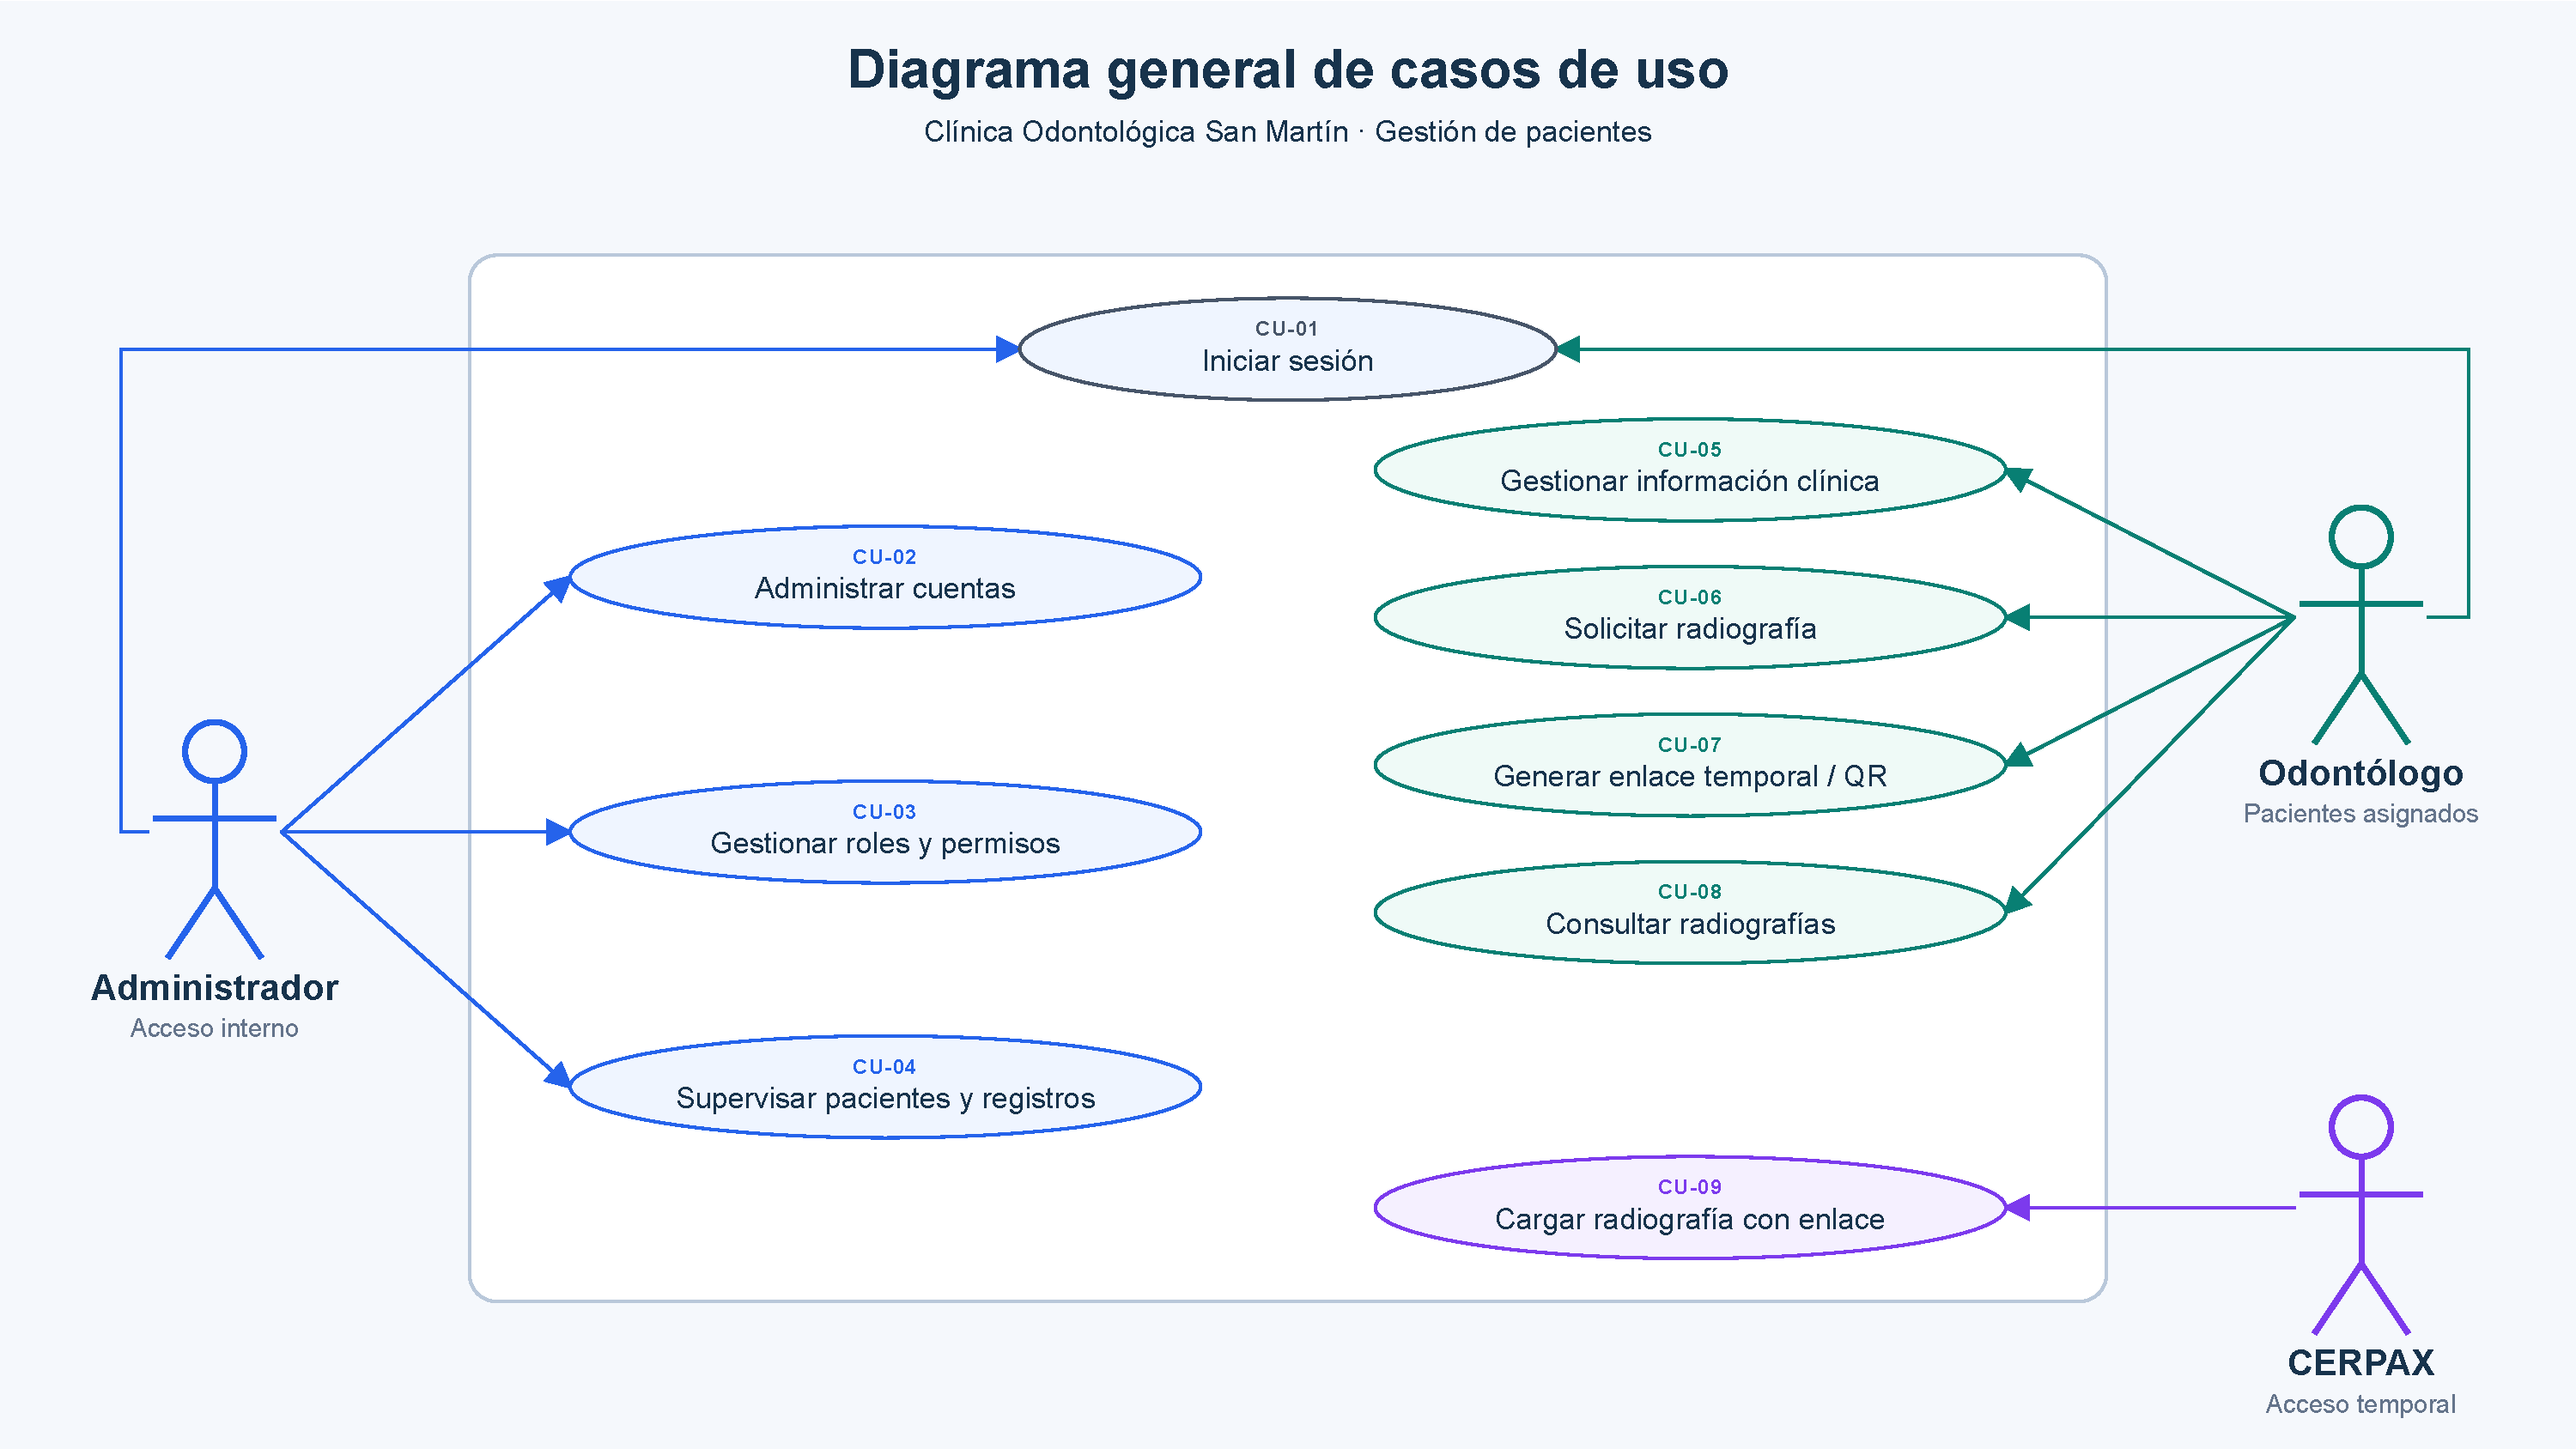
\includegraphics[
	width=\textwidth,
	keepaspectratio
	]{../diagramas/casos_de_uso.pdf}
	
	\caption{Diagrama general de casos de uso. \fuentepropia}
	\label{fig:casos-uso-general}
\end{figure}

A continuación se describen los casos de uso más relevantes representados
en el diagrama general. Para cada uno se indica el actor que participa,
la condición necesaria antes de iniciar, el flujo principal, las posibles
situaciones alternativas y el resultado esperado al finalizar la operación.

\paragraph{CU-01. Iniciar sesión}

\begin{description}
	
	\item[Actor.] Administrador y Odontólogo.
	
	\item[Precondición.] El usuario debe contar con una cuenta activa y
	credenciales válidas.
	
	\item[Flujo principal.] El usuario ingresa su correo y contraseña. El sistema
	verifica la información y, si es correcta, permite el acceso a las funciones
	disponibles según su rol.
	
	\item[Alternativas.] Si las credenciales son incorrectas o la cuenta no puede
	utilizarse, el sistema rechaza el acceso y muestra el mensaje correspondiente.
	
	\item[Postcondición.] El usuario queda autenticado y puede ingresar a las
	funciones permitidas para su perfil.
	
\end{description}


\paragraph{CU-02. Administrar cuentas}

\begin{description}
	
	\item[Actor.] Administrador.
	
	\item[Precondición.] El Administrador debe haber iniciado sesión y contar con
	los permisos necesarios.
	
	\item[Flujo principal.] El Administrador accede al módulo de usuarios,
	consulta las cuentas existentes y realiza las operaciones permitidas para
	registrar o modificar la información de una cuenta.
	
	\item[Alternativas.] Si los datos ingresados no son válidos, el sistema
	rechaza la operación e informa el error.
	
	\item[Postcondición.] La cuenta queda registrada o actualizada de acuerdo con
	la operación realizada.
	
\end{description}


\paragraph{CU-03. Gestionar roles y permisos}

\begin{description}
	
	\item[Actor.] Administrador.
	
	\item[Precondición.] El Administrador debe encontrarse autenticado.
	
	\item[Flujo principal.] El Administrador accede a la gestión de roles y
	permisos, selecciona el usuario correspondiente y realiza los cambios
	permitidos.
	
	\item[Alternativas.] Si la operación no está autorizada o la información no
	es válida, el sistema rechaza el cambio.
	
	\item[Postcondición.] La configuración de acceso del usuario queda actualizada.
	
\end{description}


\paragraph{CU-04. Supervisar pacientes y registros}

\begin{description}
	
	\item[Actor.] Administrador.
	
	\item[Precondición.] El Administrador debe haber iniciado sesión y contar con
	acceso a los módulos correspondientes.
	
	\item[Flujo principal.] El Administrador consulta los registros disponibles
	relacionados con pacientes y con las funciones administrativas permitidas.
	
	\item[Alternativas.] Si intenta acceder a información para la cual no dispone
	de permiso, el sistema rechaza la solicitud.
	
	\item[Postcondición.] La información permitida queda disponible para su
	consulta.
	
\end{description}


\paragraph{CU-05. Gestionar información clínica}

\begin{description}
	
	\item[Actor.] Odontólogo.
	
	\item[Precondición.] El Odontólogo debe haber iniciado sesión y contar con
	acceso al paciente correspondiente.
	
	\item[Flujo principal.] El Odontólogo consulta el registro del paciente y
	utiliza las funciones clínicas disponibles para revisar o actualizar la
	información relacionada con su atención.
	
	\item[Alternativas.] Si los datos ingresados no son válidos o el usuario no
	tiene acceso al registro, el sistema rechaza la operación.
	
	\item[Postcondición.] La información clínica queda consultada o actualizada.
	
\end{description}


\paragraph{CU-06. Solicitar radiografía}

\begin{description}
	
	\item[Actor.] Odontólogo.
	
	\item[Precondición.] El Odontólogo debe estar autenticado y el paciente debe
	encontrarse registrado en el sistema.
	
	\item[Flujo principal.] El Odontólogo selecciona al paciente y registra la
	solicitud del estudio radiográfico con la información requerida.
	
	\item[Alternativas.] Si los datos de la solicitud no son válidos, el sistema
	rechaza el registro.
	
	\item[Postcondición.] La solicitud queda registrada y asociada al paciente.
	
\end{description}


\paragraph{CU-07. Generar enlace temporal / QR}

\begin{description}
	
	\item[Actor.] Odontólogo.
	
	\item[Precondición.] Debe existir una solicitud radiográfica válida y el
	Odontólogo debe encontrarse autenticado.
	
	\item[Flujo principal.] El Odontólogo selecciona la solicitud y genera el
	acceso temporal que será utilizado dentro del proceso de carga de la
	radiografía.
	
	\item[Alternativas.] Si la solicitud no cumple las condiciones necesarias,
	el sistema no permite generar el acceso.
	
	\item[Postcondición.] Se dispone de un enlace temporal o código QR asociado
	a la solicitud.
	
\end{description}


\paragraph{CU-08. Consultar radiografías}

\begin{description}
	
	\item[Actor.] Odontólogo.
	
	\item[Precondición.] El Odontólogo debe haber iniciado sesión y tener acceso
	al paciente correspondiente.
	
	\item[Flujo principal.] El Odontólogo consulta las solicitudes relacionadas
	con el paciente y accede a la radiografía cuando esta se encuentra
	disponible.
	
	\item[Alternativas.] Si no existe una radiografía asociada o el usuario no
	dispone de permiso, el sistema no permite la consulta.
	
	\item[Postcondición.] La radiografía puede ser consultada por el usuario
	autorizado.
	
\end{description}


\paragraph{CU-09. Cargar radiografía con enlace}

\begin{description}
	
	\item[Actor.] CERPAX.
	
	\item[Precondición.] Debe existir un acceso temporal válido asociado a una
	solicitud radiográfica.
	
	\item[Flujo principal.] CERPAX accede mediante el enlace temporal, selecciona
	el archivo correspondiente y realiza la carga. El sistema almacena el archivo
	y lo relaciona con la solicitud.
	
	\item[Alternativas.] Si el acceso no es válido o el archivo no cumple las
	condiciones permitidas, el sistema rechaza la carga.
	
	\item[Postcondición.] La radiografía queda almacenada y asociada a la
	solicitud correspondiente.
	
\end{description}

% ============================================================
% 2.4 DISEÑO DE LA SOLUCIÓN
% ============================================================

\section{Diseño de la solución}

En esta sección se presenta la estructura general del sistema propuesto
para la Clínica Odontológica San Martín. Se describen la arquitectura,
el modelo de datos, el diseño de las interfaces y la forma en que se
organizan los servicios utilizados por la aplicación.

El diseño busca mantener separados los componentes principales del sistema,
de manera que la interfaz, la lógica del backend y la persistencia de datos
puedan evolucionar de forma independiente y mantengan una comunicación
controlada entre sí.


% ------------------------------------------------------------
% ARQUITECTURA
% ------------------------------------------------------------

\subsection{Arquitectura del sistema}


\begin{figure}[H]
	\centering
	
	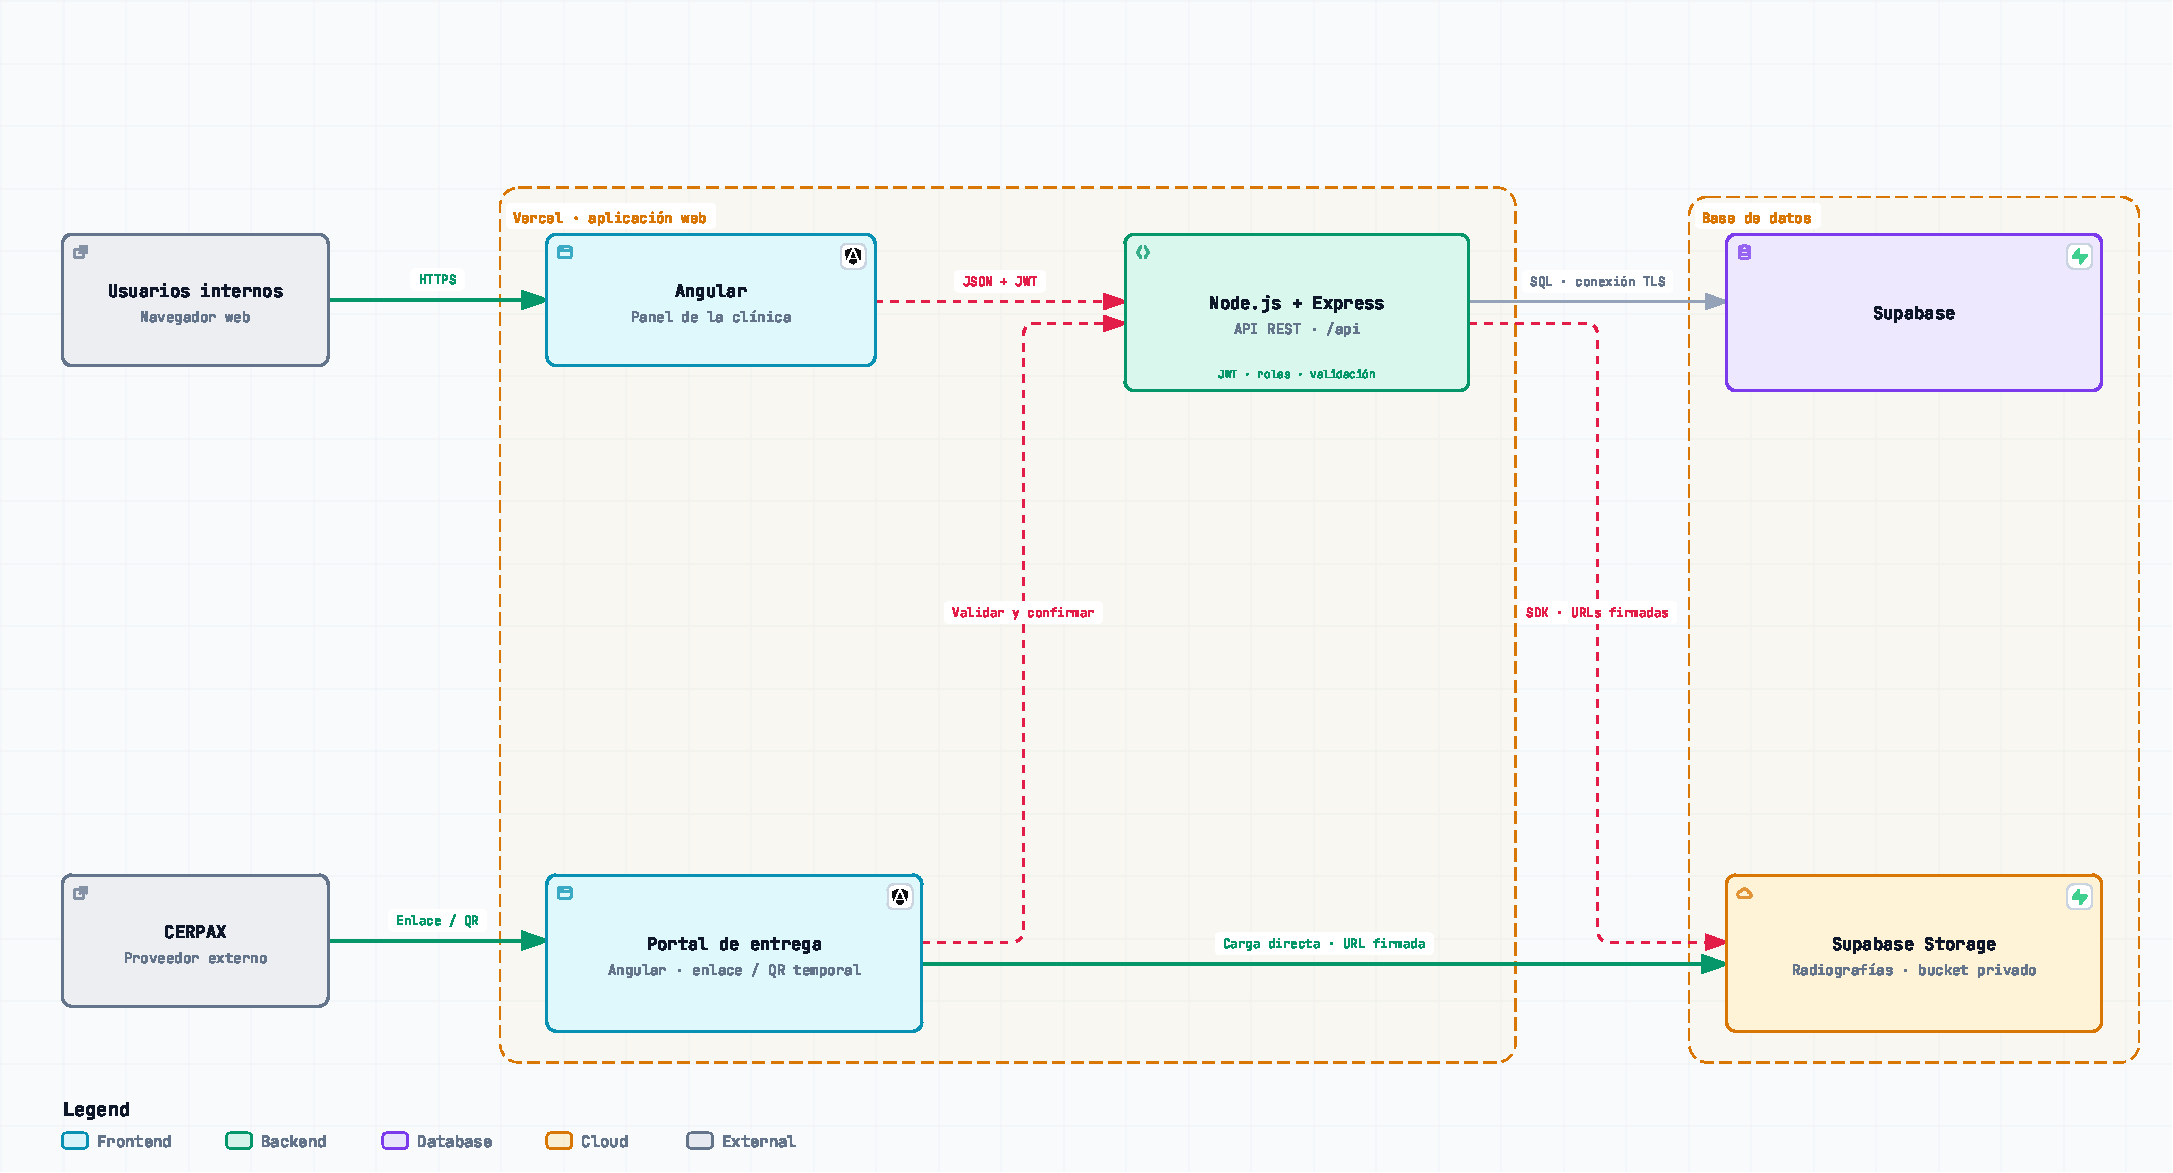
\includegraphics[
	width=0.95\textwidth,
	keepaspectratio
	]{../diagramas/arquitectura.pdf}
	
	\caption{Arquitectura general del sistema. \fuentepropia}
	\label{fig:arquitectura-sistema}
\end{figure}


%\begin{figure}[H]
%	\centering
	
%	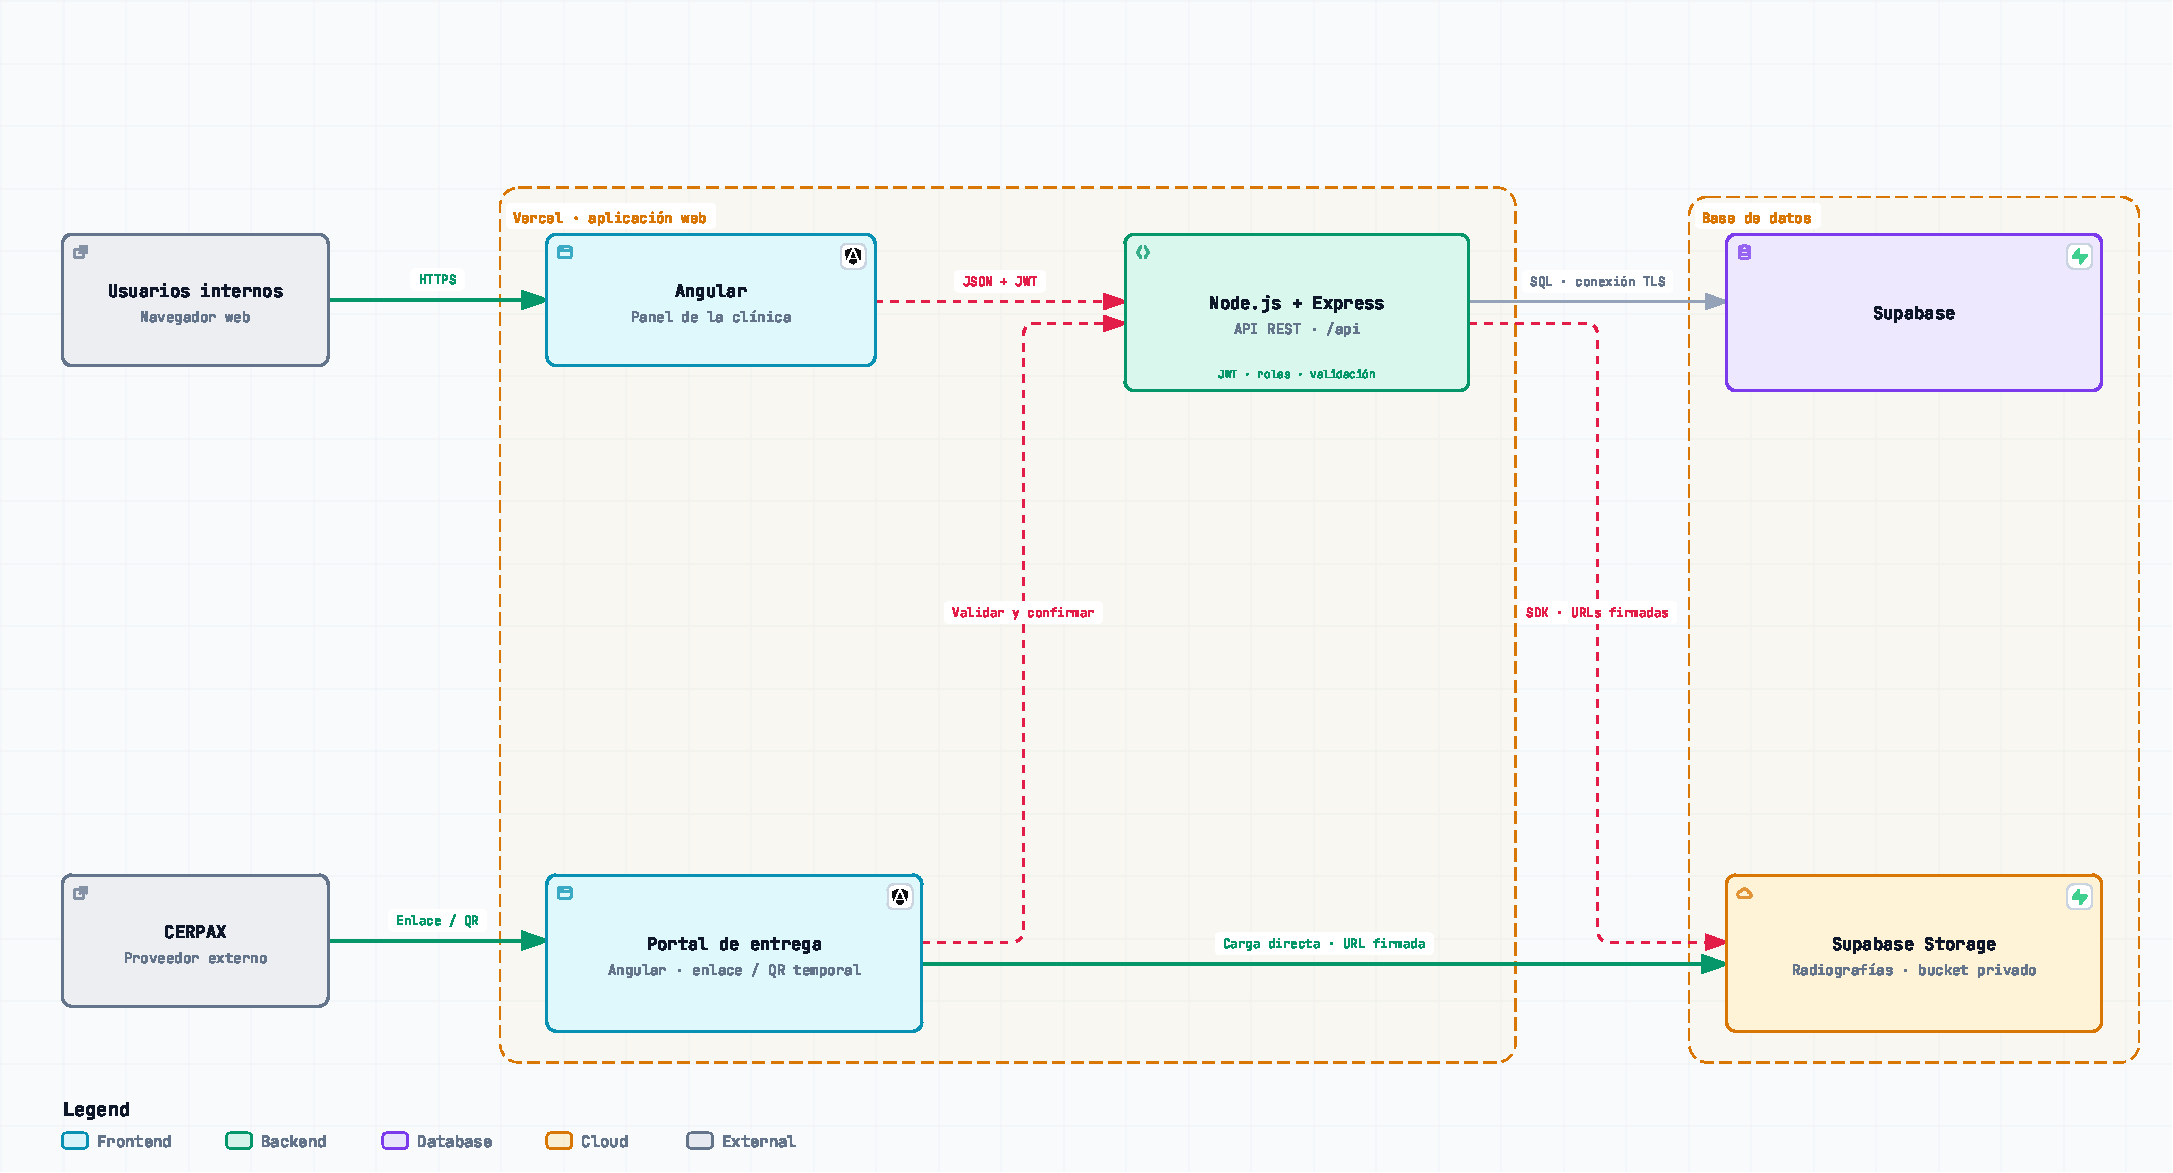
\includegraphics[
%	width=\textwidth,
%	keepaspectratio
%	]{../diagramas/arquitectura.pdf}
	
%	\caption{Arquitectura general del sistema. \fuentepropia}
%	\label{fig:arquitectura-sistema}
%\end{figure}

%La solución separa la interfaz web, la API, la base de datos y los servicios
%utilizados para almacenamiento.

%El frontend se comunica con el backend mediante HTTPS. El backend aplica las
%reglas del sistema y posteriormente realiza las operaciones necesarias sobre
%la base de datos y los servicios externos.

%\begin{figure}[H]
	
%	\centering
	
%	\begin{tikzpicture}[
%		node distance=1.3cm and 1.7cm,
%		box/.style={
%			draw,
%			rounded corners,
%			minimum width=3.4cm,
%			minimum height=1.1cm,
%			align=center
%		},
%		arr/.style={
%			-{Latex[length=2mm]},
%			thick
%		}
%		]
		
%		\node[box] (web)
%		{Aplicación web\\Angular};
		
%		\node[box,below=of web] (api)
%		{API\\Node.js + Express};
		
%		\node[box,below left=of api] (db)
%		{Supabase\\PostgreSQL};
		
%		\node[box,below right=of api] (storage)
%		{Almacenamiento\\de archivos};
		
%		\node[box,right=of api] (externo)
%		{Servicios /\\actor externo};
		
%		\draw[arr] (web) -- node[right]{HTTPS} (api);
%		\draw[arr] (api) -- (db);
%		\draw[arr] (api) -- (storage);
%		\draw[arr] (externo) -- (api);
		
%	\end{tikzpicture}
	
%	\caption{Arquitectura general del sistema. \fuentepropia}
	
%\end{figure}


% ------------------------------------------------------------
% MODELO DE DATOS
% ------------------------------------------------------------

\subsection{Modelo de datos}

El modelo de datos del sistema está implementado sobre PostgreSQL mediante
Supabase. Para facilitar su lectura, se presenta en tres partes: el núcleo
clínico, el proceso de solicitudes y radiografías, y la estructura de
cuentas, roles y permisos.

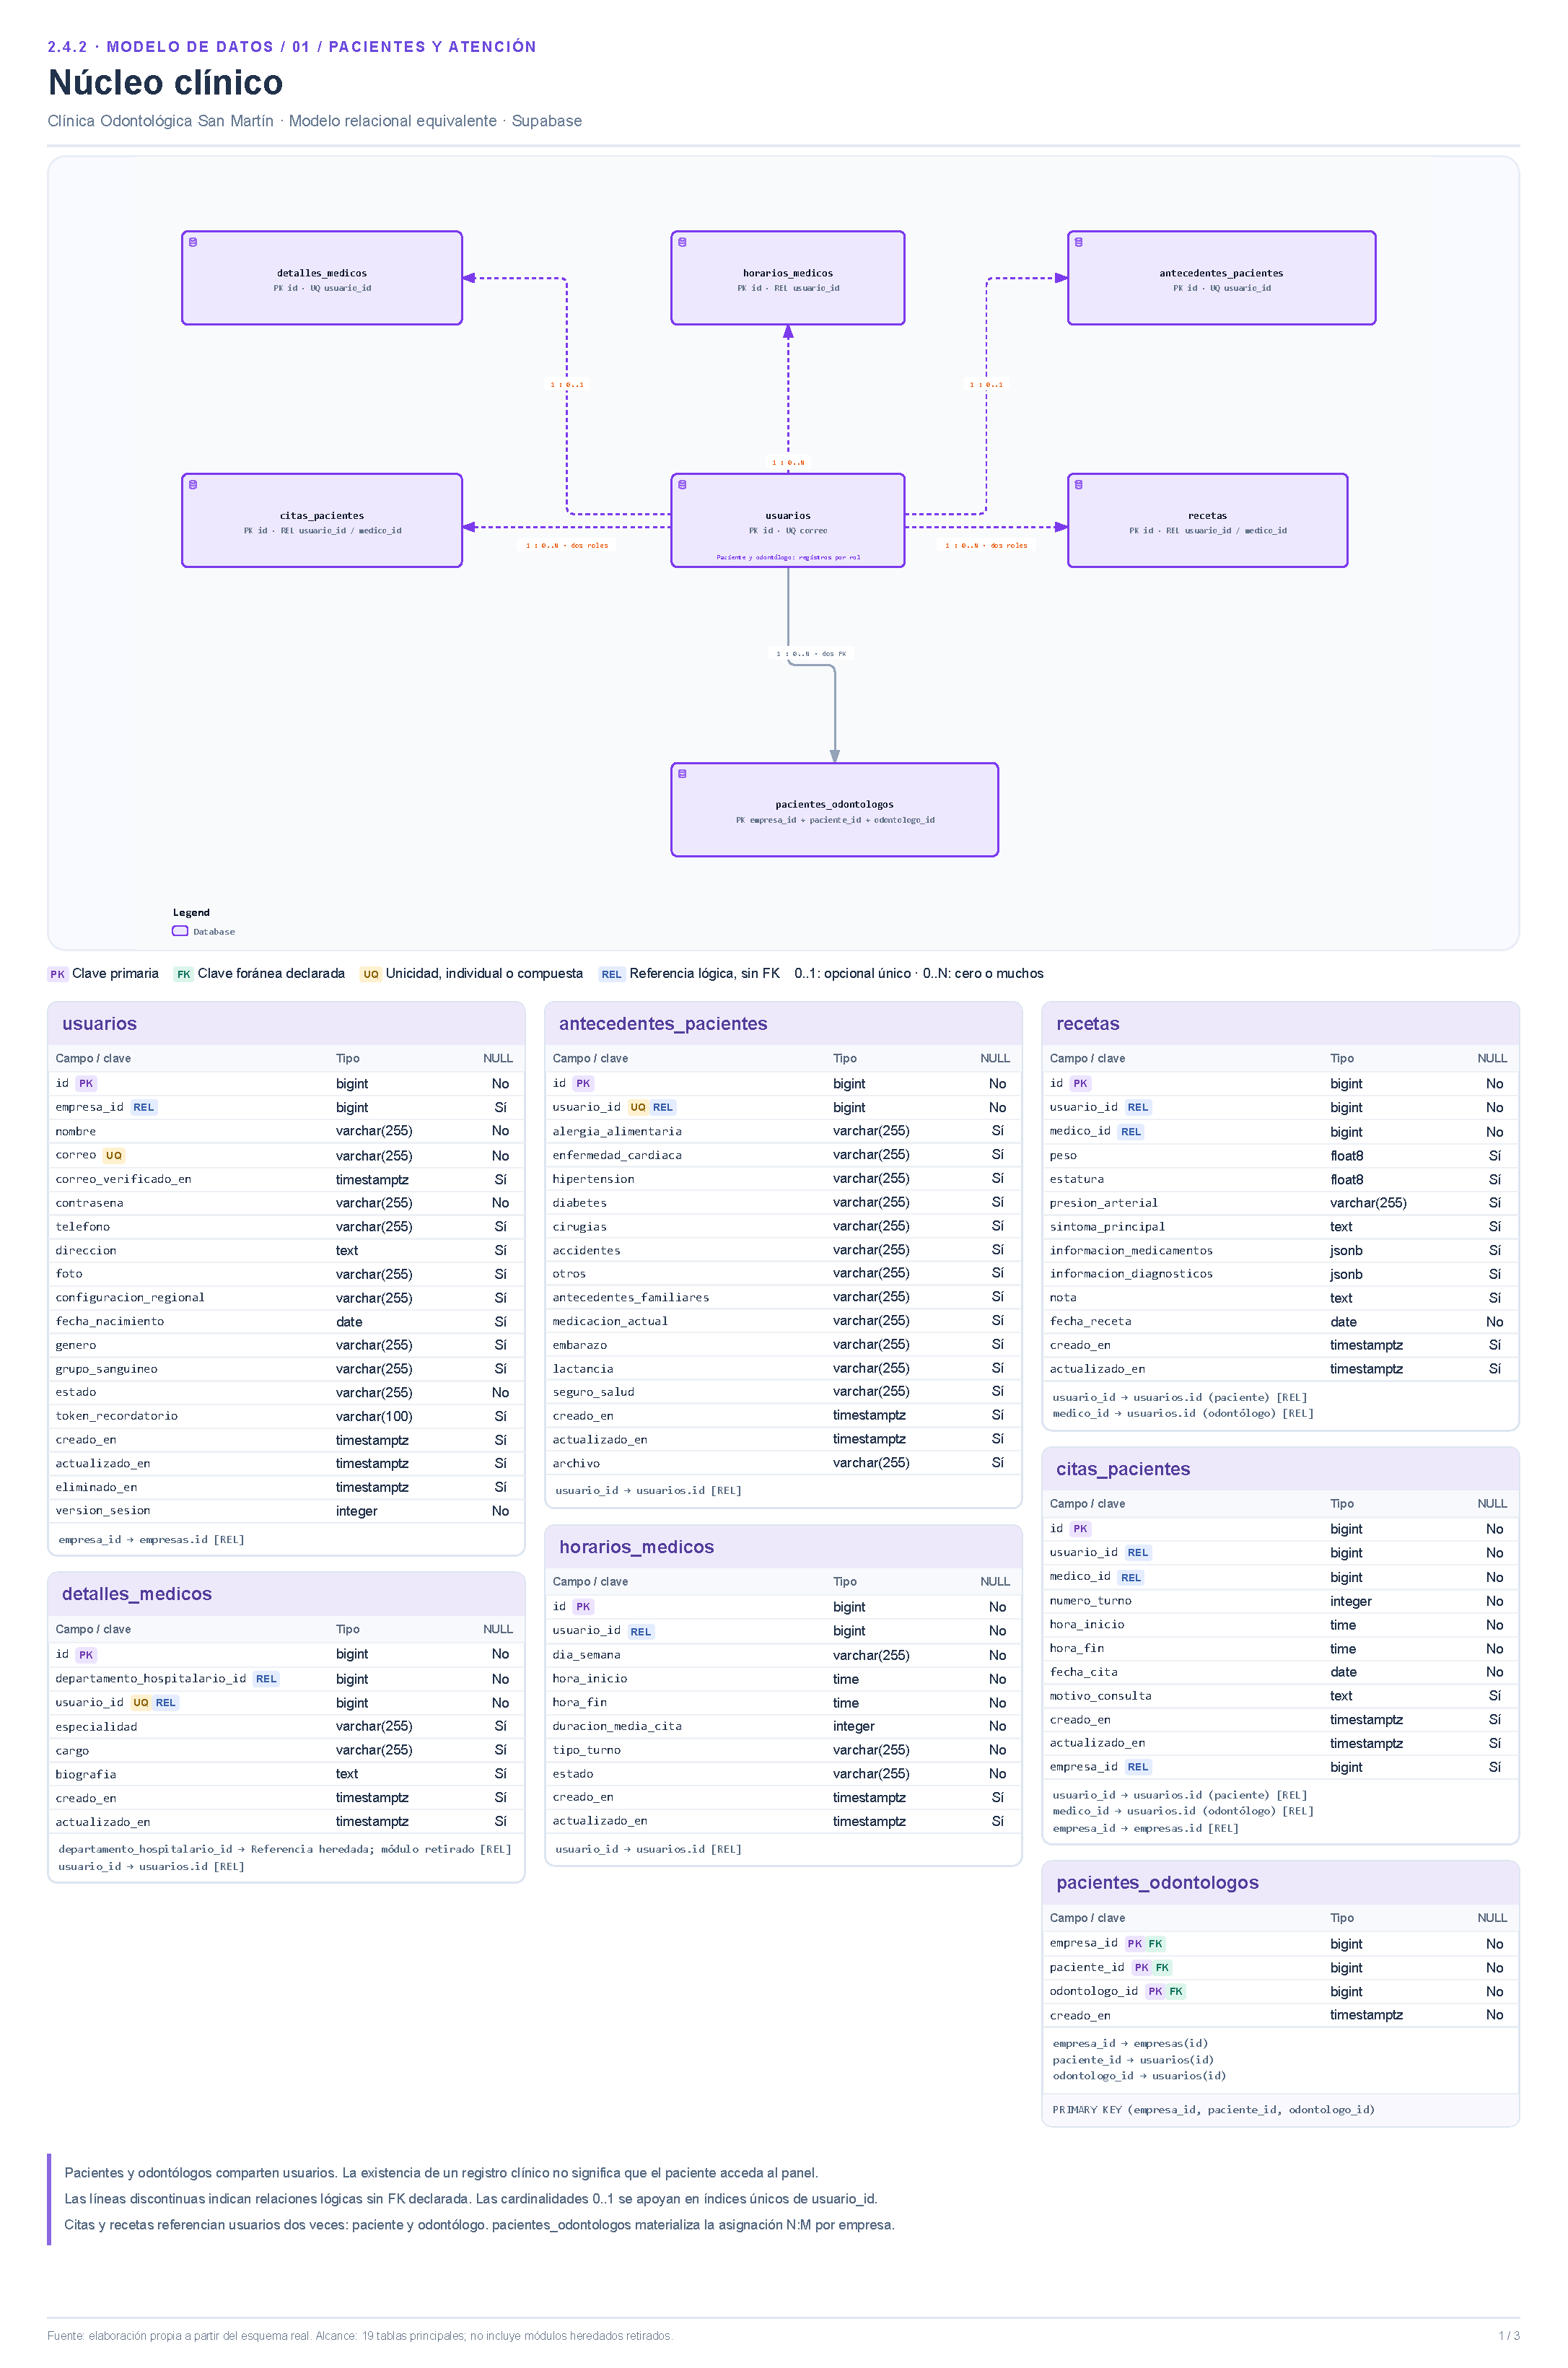
\includepdf[
pages=1-3,
pagecommand={\thispagestyle{plain}}
]{../diagramas/modelo_datos.pdf}


	\begin{table}[htbp]
		\centering
		\caption{Diccionario de datos de la entidad
			\texttt{solicitudes\_radiografias}}
		\label{tab:diccionario-solicitudes}
		
		\small
		\renewcommand{\arraystretch}{1.25}
		\setlength{\tabcolsep}{4pt}
		
		\begin{tabularx}{\textwidth}{
				>{\raggedright\arraybackslash}p{0.23\textwidth}
				>{\raggedright\arraybackslash}p{0.20\textwidth}
				>{\centering\arraybackslash}p{0.07\textwidth}
				>{\raggedright\arraybackslash}X
			}
			\toprule
			\textbf{Campo} &
			\textbf{Tipo} &
			\textbf{Nulo} &
			\textbf{Descripción y reglas} \\
			\midrule
			
			\texttt{id} &
			BIGINT &
			No &
			Identificador único de la solicitud.
			Clave primaria (PK). \\
			
			\texttt{empresa\_id} &
			BIGINT &
			No &
			Clínica a la que pertenece la solicitud.
			Clave foránea (FK) hacia \texttt{empresas.id}. \\
			
			\texttt{paciente\_id} &
			BIGINT &
			No &
			Paciente para quien se solicita la radiografía.
			Clave foránea hacia \texttt{usuarios.id}. \\
			
			\texttt{odontologo\_id} &
			BIGINT &
			No &
			Odontólogo responsable de la solicitud.
			Clave foránea hacia \texttt{usuarios.id}. \\
			
			\texttt{tipo} &
			VARCHAR(150) &
			No &
			Tipo de estudio radiográfico solicitado.
			Admite hasta 150 caracteres. \\
			
			\texttt{indicaciones} &
			VARCHAR(2000) &
			No &
			Instrucciones para realizar el estudio.
			Admite hasta 2000 caracteres; puede contener
			una cadena vacía. \\
			
			\texttt{estado} &
			TEXT &
			No &
			Situación de la solicitud. La restricción
			CHECK permite únicamente:
			\textit{Pendiente}, \textit{Completada}
			o \textit{Cancelada}. \\
			
			\texttt{creado\_en} &
			TIMESTAMPTZ &
			No &
			Fecha y hora de creación de la solicitud,
			con información de zona horaria. \\
			
			\texttt{completado\_en} &
			TIMESTAMPTZ &
			Sí &
			Fecha y hora de finalización del estudio.
			Puede permanecer nulo mientras la solicitud
			no se haya completado. \\
			
			\bottomrule
		\end{tabularx}
		
		\vspace{3pt}
		{\footnotesize\textit{Fuente: Elaboración propia
				a partir del esquema de la base de datos del sistema.}}
	\end{table}


% TODO IMAGEN OBLIGATORIA:
% Crear modelo entidad-relación a partir de las tablas REALES.
%
% Archivo sugerido:
% figuras/modelo-er.png


% ------------------------------------------------------------
% INTERFAZ
% ------------------------------------------------------------

\subsection{Diseño de la interfaz}

\begin{figure}[H]
	\centering
	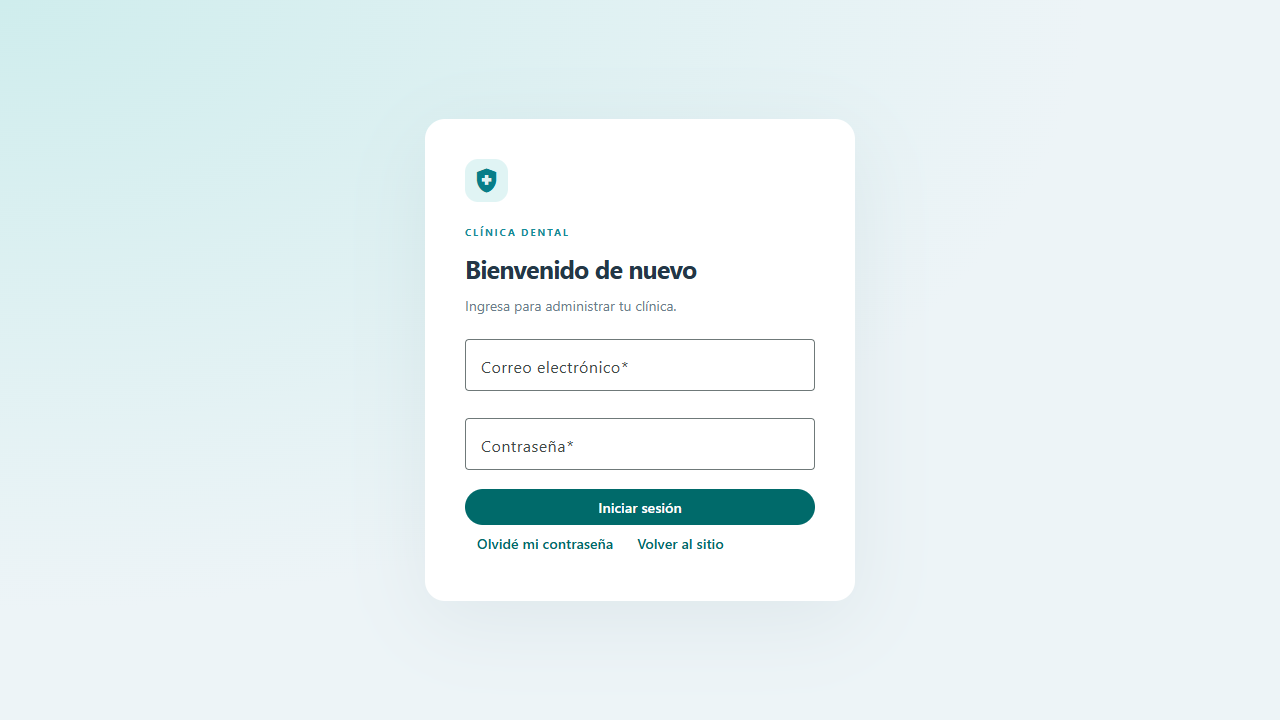
\includegraphics[
	width=0.95\textwidth,
	keepaspectratio
	]{../../evidencia/login-prueba.png}
	
	\caption{Módulo login en vista de escritorio. \fuentepropia}
	\label{fig:login-escritorio}
\end{figure}

\begin{figure}[H]
	\centering
	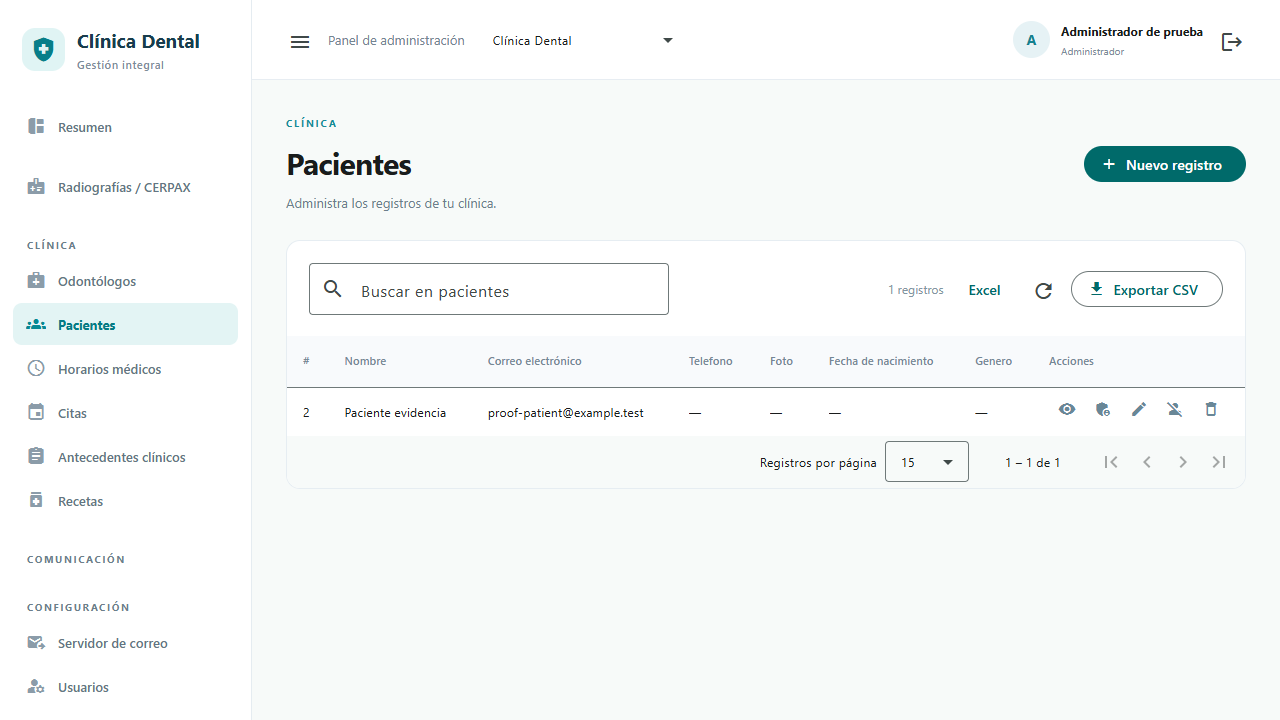
\includegraphics[
	width=0.95\textwidth,
	keepaspectratio
	]{../../evidencia/pacientes-prueba.png}
	
	\caption{Módulo de gestión de pacientes en vista de escritorio. \fuentepropia}
	\label{fig:pacientes-escritorio}
\end{figure}

\begin{figure}[H]
	\centering
	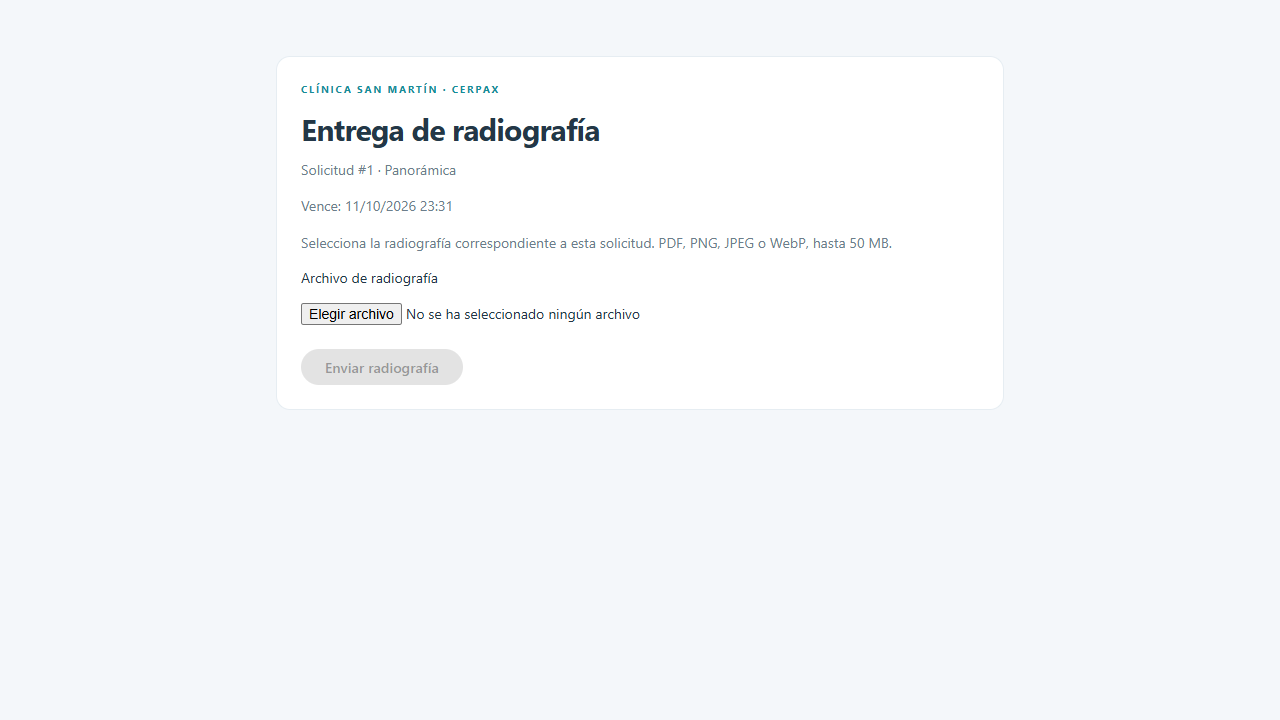
\includegraphics[
	width=0.95\textwidth,
	keepaspectratio
	]{../../evidencia/portal-cerpax-prueba.png}
	
	\caption{Portal externo de entrega CERPAX. \fuentepropia}
	\label{fig:cerpax}
\end{figure}

\begin{figure}[H]
	\centering
	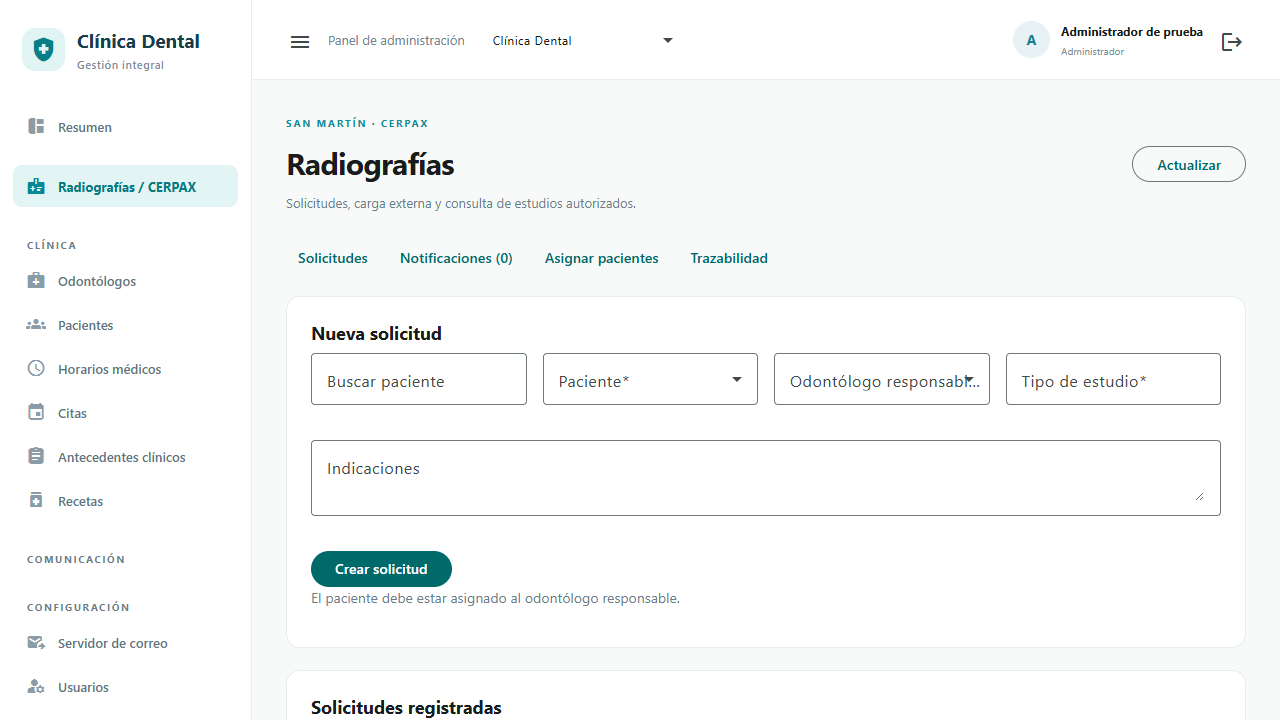
\includegraphics[
	width=0.95\textwidth,
	keepaspectratio
	]{../../evidencia/solicitudes-prueba.png}
	
	\caption{Gestión de solicitudes radiográficas. \fuentepropia}
	\label{fig:solicitudes-escritorio}
\end{figure}

% TODO IMÁGENES:
%
% figuras/login-escritorio.png
% figuras/login-movil.png
% figuras/pacientes-escritorio.png
% figuras/pacientes-movil.png
% figuras/citas.png
% figuras/solicitud-radiografia.png

%\imagenopcional
%{figuras/login-escritorio.png}
%{0.85}
%{Pantalla de inicio de sesión en escritorio.}
%{fig:login-escritorio}

%\imagenopcional
%{figuras/pacientes-escritorio.png}
%{0.85}
%{Pantalla de gestión de pacientes.}
%{fig:pacientes-escritorio}
\subsection{Diseño de la interfaz de programación de aplicaciones}
% En el preámbulo:
% \usepackage{booktabs,longtable,array,url}

\begingroup
\small
\renewcommand{\arraystretch}{1.2}
\setlength{\tabcolsep}{4pt}

\begin{longtable}{@{}
		>{\raggedright\arraybackslash}p{0.09\linewidth}
		>{\raggedright\arraybackslash}p{0.29\linewidth}
		>{\raggedright\arraybackslash}p{0.39\linewidth}
		>{\raggedright\arraybackslash}p{0.15\linewidth}@{}}
	
	\caption{Diseño de endpoints principales}
	\label{tab:endpoints-principales}\\
	
	\toprule
	\textbf{Método} &
	\textbf{Ruta} &
	\textbf{Propósito y parámetros} &
	\textbf{Respuestas} \\
	\midrule
	\endfirsthead
	
	\multicolumn{4}{c}{\tablename\ \thetable\ (continuación)}\\
	\toprule
	\textbf{Método} &
	\textbf{Ruta} &
	\textbf{Propósito y parámetros} &
	\textbf{Respuestas} \\
	\midrule
	\endhead
	
	\midrule
	\multicolumn{4}{r}{Continúa en la siguiente página.}\\
	\endfoot
	
	\bottomrule
	\endlastfoot
	
	POST &
	\path{/api/v1/login} &
	Autentica mediante \texttt{correo} y \texttt{contrasena}. Devuelve un token
	JWT y los datos del usuario. &
	200, 400, 401, 429 \\
	
	GET &
	\path{/api/v1/pacientes} &
	Lista los pacientes autorizados. Parámetros de consulta opcionales:
	\texttt{page}, \texttt{size} y \texttt{search}. &
	200, 401, 403 \\
	
	POST &
	\path{/api/v1/pacientes} &
	Registra un paciente. Recibe \texttt{nombre}, \texttt{correo} y los demás
	campos permitidos por el catálogo y el rol. &
	201, 401, 403, 422 \\
	
	GET &
	\path{/api/v1/radiographs} &
	Consulta solicitudes autorizadas. Filtros opcionales:
	\texttt{paciente}, \texttt{estado} y \texttt{page}. &
	200, 401, 403, 422 \\
	
	POST &
	\path{/api/v1/radiographs} &
	Crea una solicitud con \texttt{paciente\_id}, \texttt{tipo} e
	\texttt{indicaciones}. El administrador también indica
	\texttt{odontologo\_id}. &
	201, 401, 403, 404, 422 \\
	
	POST &
	\path{/api/v1/radiographs/:id/access} &
	Genera un enlace temporal y un código QR. Recibe el identificador de la
	solicitud y \texttt{horas}, entre 1 y 72; el valor predeterminado es 24. &
	201, 401, 403, 404, 409, 422 \\
	
	GET &
	\path{/api/v1/radiographs/:id/file} &
	Permite acceder al archivo de una solicitud autorizada. El parámetro opcional
	\texttt{download=1} solicita la descarga del archivo. &
	200, 302, 401, 403, 404, 422, 503 \\
	
	POST &
	\path{/api/v1/external/radiographs/access} &
	Valida el \texttt{token} del enlace temporal utilizado por CERPAX, sin
	requerir inicio de sesión. Devuelve los datos mínimos de la solicitud y
	su vencimiento. &
	200, 410, 429 \\
	
	POST &
	\path{/api/v1/external/radiographs/upload-url} &
	Prepara la carga del archivo mediante una URL firmada. Recibe
	\texttt{token}, \texttt{nombre}, \texttt{tipo} MIME y \texttt{tamano}
	en bytes. &
	200, 410, 422, 429, 503 \\
	
	POST &
	\path{/api/v1/external/radiographs/upload-complete} &
	Confirma la carga realizada en Supabase Storage. Recibe \texttt{token},
	\texttt{path}, \texttt{nombre}, \texttt{tipo} y \texttt{tamano}.
	Al completarse correctamente, la solicitud queda asociada con la radiografía. &
	201, 409, 410, 422, 429 \\
	
\end{longtable}

\noindent\textit{Fuente: Elaboración propia a partir de las rutas
	implementadas en el sistema.}

\medskip

\noindent
Las rutas internas protegidas requieren el encabezado
\texttt{Authorization: Bearer <JWT>} y los permisos correspondientes.
Las rutas externas utilizadas para la carga de radiografías emplean un
token temporal. Un acceso sin autorización puede generar una respuesta
403, mientras que los errores internos del servidor pueden producir una
respuesta 500. El código 400 se utiliza, entre otros casos, cuando faltan
datos requeridos durante la autenticación o estos presentan un tipo
incorrecto; para las validaciones de los datos enviados al sistema se
utiliza principalmente el código 422.

\endgroup

\section{Justificación del stack tecnológico}

\begingroup
\small
\renewcommand{\arraystretch}{1.2}
\setlength{\tabcolsep}{4pt}

\begin{longtable}{@{}
		>{\raggedright\arraybackslash}p{0.21\linewidth}
		>{\raggedright\arraybackslash}p{0.15\linewidth}
		>{\raggedright\arraybackslash}p{0.23\linewidth}
		>{\raggedright\arraybackslash}p{0.33\linewidth}@{}}
	
	\caption{Stack tecnológico y justificación de selección}
	\label{tab:stack-tecnologico}\\
	
	\toprule
	\textbf{Componente} &
	\textbf{Versión} &
	\textbf{Función} &
	\textbf{Criterio de selección} \\
	\midrule
	\endfirsthead
	
	\multicolumn{4}{c}{\tablename\ \thetable\ (continuación)}\\
	\toprule
	\textbf{Componente} &
	\textbf{Versión} &
	\textbf{Función} &
	\textbf{Criterio de selección} \\
	\midrule
	\endhead
	
	\midrule
	\multicolumn{4}{r}{Continúa en la siguiente página.}\\
	\endfoot
	
	\bottomrule
	\endlastfoot
	
	Angular &
	21.2.23 &
	Interfaz web de gestión clínica. &
	Permite organizar formularios, navegación y vistas mediante componentes
	reutilizables para la administración de pacientes, usuarios y solicitudes
	radiográficas. \\
	
	TypeScript &
	5.9.3 &
	Lenguaje de implementación del frontend web. &
	El tipado estático ayuda a detectar inconsistencias entre formularios,
	modelos y respuestas de la API durante el desarrollo. \\
	
	Angular Material &
	21.2.14 &
	Componentes visuales de la aplicación web. &
	Proporciona controles reutilizables para formularios, tablas, diálogos y
	navegación, permitiendo mantener una interfaz uniforme entre los distintos
	módulos del sistema. \\
	
	Node.js / Express &
	24.16.0 / 5.2.1 &
	API HTTP, validaciones y lógica de negocio. &
	Permite centralizar la autenticación, la autorización, las validaciones y el
	acceso a los datos desde una misma capa de backend. \\
	
	PostgreSQL en Supabase &
	17.6 &
	Persistencia de datos clínicos y administrativos. &
	El modelo relacional permite representar pacientes, odontólogos, solicitudes,
	accesos temporales y demás entidades mediante claves y restricciones que
	favorecen la consistencia de la información. \\
	
	Supabase Storage &
	Servicio administrado; SDK JavaScript 2.117.2 &
	Almacenamiento de archivos radiográficos. &
	Permite mantener los archivos radiográficos separados de sus metadatos
	relacionales y utilizar mecanismos de acceso controlado mediante URL firmadas. \\
	
	jsonwebtoken / bcryptjs &
	9.0.3 / 3.0.3 &
	Gestión de sesiones y verificación de contraseñas. &
	JWT permite identificar sesiones autenticadas en las solicitudes dirigidas
	a la API, mientras que bcryptjs permite verificar contraseñas mediante hashes.
	Las autorizaciones se validan en el backend según el rol y los permisos
	asignados. \\
	
	Vercel &
	Plataforma administrada &
	Despliegue de la aplicación web y su API. &
	Permite publicar la aplicación y mantener disponible el frontend junto con
	los servicios necesarios para la comunicación con el backend. \\
	
	Git / GitHub &
	Git 2.44.0.windows.1; GitHub como servicio &
	Control de versiones y alojamiento del repositorio. &
	Permite conservar el historial de cambios del código fuente, la documentación,
	las migraciones y demás archivos del proyecto, facilitando el seguimiento del
	desarrollo y la recuperación de versiones anteriores. \\
	
\end{longtable}

\vspace{0.2cm}

\noindent\textit{Fuente: Elaboración propia a partir del código,
	las dependencias del proyecto, el entorno de desarrollo y los metadatos
	de la base de datos.}

\endgroup


% ------------------------------------------------------------
% API
% ------------------------------------------------------------


% ============================================================
% 2.6 IMPLEMENTACIÓN
% ============================================================

\section{Implementación}

La implementación del sistema se orientó a integrar en una misma solución
los procesos de gestión de pacientes y el manejo de solicitudes radiográficas
de la Clínica Odontológica San Martín. Para ello se desarrolló una aplicación
web conectada a una API, una base de datos relacional y un servicio de
almacenamiento destinado a los archivos radiográficos.

La aplicación fue organizada de manera que las responsabilidades de la
interfaz, la lógica de negocio, la persistencia de datos y el almacenamiento
de archivos permanecieran separadas. Esta decisión facilitó el desarrollo de
los distintos módulos y permitió mantener un control más claro sobre la
información utilizada por el sistema.

\subsection{Implementación de la plataforma web}

La interfaz web fue desarrollada con Angular y TypeScript. Para mantener una
apariencia uniforme entre los distintos módulos se utilizaron componentes de
Angular Material en formularios, tablas, diálogos y elementos de navegación.

Desde la aplicación web se gestionan los registros utilizados en la actividad
de la clínica, entre ellos pacientes, odontólogos, horarios, citas y
antecedentes clínicos. La interfaz se comunica con el backend mediante
solicitudes HTTP y muestra las opciones disponibles de acuerdo con las
funciones correspondientes al usuario autenticado.

El paciente se maneja dentro del sistema como un registro clínico y no como
un usuario que inicia sesión. Los perfiles internos con acceso al sistema son
Administrador y Odontólogo. Esta separación permite mantener las funciones
administrativas y clínicas dentro de los usuarios autorizados sin crear
cuentas adicionales para los pacientes.

La digitalización de este tipo de procesos coincide con propuestas recientes
que plantean el uso de sistemas informáticos para centralizar información de
pacientes y actividades de gestión dentro de clínicas odontológicas
\parencite{ho2024}.

\subsection{Implementación del backend}

El backend fue desarrollado con Node.js y Express. Este componente concentra
la lógica de negocio y actúa como intermediario entre la aplicación web y los
servicios de persistencia utilizados por el sistema.

Las solicitudes realizadas desde el frontend son procesadas por la API antes
de acceder a la información almacenada. De esta manera, las validaciones y
restricciones de acceso no dependen únicamente de la interfaz, sino que
también son comprobadas en el servidor.

La separación entre frontend y backend permitió mantener las reglas de negocio
fuera de los componentes visuales y disponer de un punto central desde el cual
gestionar la autenticación, los permisos y el acceso a los datos.

\subsection{Gestión de pacientes y odontólogos}

La información de pacientes y odontólogos se almacena de manera estructurada
en PostgreSQL. Ambos forman parte del modelo de usuarios del sistema, pero su
participación se diferencia mediante las relaciones y funciones establecidas
en la base de datos.

Para representar la relación entre un paciente y el profesional responsable
se utiliza una asociación específica dentro del modelo de datos. Esta
estructura permite organizar los registros clínicos y conservar la relación
entre el paciente, el odontólogo y la clínica correspondiente.

La gestión de pacientes contempla operaciones de registro, consulta y
actualización de información. En el caso del odontólogo, además de sus datos
generales, el sistema mantiene la relación con los pacientes y demás elementos
necesarios para la atención clínica.

\subsection{Implementación del flujo radiográfico}

Una de las funcionalidades principales del proyecto corresponde a la gestión
de solicitudes radiográficas. El proceso comienza cuando el odontólogo
registra una solicitud asociada a un paciente, indicando el tipo de estudio y
las indicaciones necesarias.

Las solicitudes mantienen un estado que permite conocer su situación dentro
del proceso. En el modelo se contemplan los estados \textit{Pendiente},
\textit{Completada} y \textit{Cancelada}.

Para evitar que el paciente tenga que actuar como intermediario digital entre
el odontólogo y CERPAX, el sistema incorpora un mecanismo de acceso temporal.
A partir de una solicitud puede generarse un enlace que puede representarse
también mediante un código QR.

CERPAX utiliza este acceso sin iniciar sesión dentro de la plataforma. De esta
manera, su participación se limita a la entrega del archivo correspondiente a
la solicitud para la cual se generó el acceso.

La base de datos mantiene información asociada a estos accesos temporales,
incluyendo datos relacionados con su vencimiento, revocación y utilización.
Una solicitud puede disponer de varios accesos temporales a lo largo de su
ciclo de vida, mientras que el modelo establece una única radiografía asociada
a cada solicitud.

\subsection{Almacenamiento de las radiografías}

Una de las decisiones técnicas adoptadas durante la implementación fue separar
los archivos radiográficos de la información almacenada directamente en la
base de datos.

Los archivos se gestionan mediante Supabase Storage, mientras que PostgreSQL
conserva los datos necesarios para relacionar cada radiografía con su
solicitud. Para ello se mantiene una referencia a la ubicación del archivo
dentro del servicio de almacenamiento.

Esta decisión permite que la base de datos se concentre en la información
estructurada del sistema y evita almacenar directamente los archivos
radiográficos dentro de las tablas principales.

El sistema contempla archivos en formatos PDF, PNG, JPEG y WebP. De acuerdo
con las restricciones definidas para este proceso, el tamaño máximo permitido
para un archivo radiográfico es de 50 MiB.

El uso de herramientas digitales para el manejo de información radiográfica
forma parte de una tendencia más amplia de incorporación de tecnologías en
los procesos odontológicos . En este
proyecto, sin embargo, las radiografías se utilizan únicamente para su
almacenamiento, asociación y consulta; el sistema no realiza diagnóstico
automático de imágenes.

\subsection{Control de acceso}

El sistema diferencia las funciones disponibles para los perfiles de
Administrador y Odontólogo.

El Administrador dispone de las operaciones necesarias para la gestión de
cuentas, roles y permisos, además de las funciones administrativas definidas
para la clínica. Por su parte, el Odontólogo utiliza las funciones relacionadas
con la gestión clínica, los pacientes que le corresponden y las solicitudes
radiográficas.

El paciente no dispone de acceso autenticado al sistema. Del mismo modo,
CERPAX no cuenta con un usuario interno, ya que su participación se realiza
mediante el acceso temporal asociado a una solicitud.

Esta decisión permitió reducir la cantidad de actores que requieren acceso
directo al sistema y mantener separados los procesos internos de la clínica
de la participación del proveedor externo.

\subsection{Dificultades encontradas y decisiones de implementación}

Una de las principales dificultades fue relacionar de manera consistente una
solicitud radiográfica con el archivo recibido posteriormente. La solicitud y
la radiografía se generan en momentos diferentes del proceso, por lo que fue
necesario conservar una relación que permitiera identificar a qué solicitud
corresponde cada archivo.

Para resolver este problema se separó el proceso en distintas etapas: registro
de la solicitud, generación del acceso temporal, carga del archivo y
asociación de la radiografía con la solicitud correspondiente. Esta separación
permitió representar cada etapa dentro del modelo de datos y controlar mejor
el flujo de información.

Otra dificultad fue determinar cómo permitir que CERPAX entregue una
radiografía sin otorgarle una cuenta dentro del sistema. La solución adoptada
consistió en utilizar accesos temporales vinculados a una solicitud concreta.
De esta forma, el proveedor externo puede participar en el proceso sin acceder
al panel interno de la clínica.

También fue necesario diferenciar claramente al paciente de los usuarios que
utilizan la plataforma. Aunque el paciente forma parte central de la
información clínica, se decidió manejarlo como un registro del sistema y no
como un perfil autenticado. Los perfiles clínicos y administrativos principales son Administrador y
Odontólogo; existe además Recepcionista con permisos administrativos
limitados, descritos en la matriz de autorización.

Otra decisión técnica relevante fue utilizar un servicio específico para el
almacenamiento de radiografías en lugar de guardar los archivos directamente
en PostgreSQL. Esta separación facilita el manejo de los archivos y mantiene
en la base de datos únicamente la información necesaria para relacionarlos
con el resto del sistema.

\subsection{Control de versiones de la implementación}

El código fuente del proyecto se mantiene bajo control de versiones mediante
Git y GitHub. El repositorio conserva los cambios realizados durante el
desarrollo, junto con los archivos de configuración, scripts y migraciones
utilizados por el sistema.

El uso de control de versiones permite mantener un historial del desarrollo y
facilita la revisión de los cambios realizados en cada etapa. El código
completo se encuentra disponible en el repositorio indicado en los anexos de
este documento.

En esta sección se describen únicamente las funcionalidades y decisiones
necesarias para comprender la implementación. Los aspectos específicos de
seguridad se desarrollan en la Sección~2.7 y los resultados de las pruebas se
presentan en la Sección~2.8.

\subsection{Estructura del proyecto}

El proyecto web se organiza en carpetas que separan la interfaz, los
servicios del servidor, la estructura de datos y la documentación. Esta
distribución permite identificar la responsabilidad de cada componente y
realizar cambios sin concentrar toda la implementación en un único archivo.

El archivo \texttt{package.json} ubicado en la raíz define la configuración
general del proyecto, los espacios de trabajo del frontend y del backend, así
como los comandos utilizados para la ejecución, compilación y pruebas.

Las carpetas principales tienen las siguientes responsabilidades:

\begin{itemize}
	
	\item \texttt{frontend/}: contiene la aplicación web desarrollada con
	Angular. En \texttt{src/app/} se encuentran las vistas y componentes
	relacionados con el inicio de sesión, pacientes, odontólogos,
	radiografías, perfil y configuración. El archivo \texttt{api.ts}
	concentra la comunicación HTTP con el backend y el manejo de la sesión.
	Los componentes relacionados con radiografías permiten interactuar con
	las solicitudes, mientras que la interfaz externa se utiliza para el
	proceso de entrega realizado mediante el acceso temporal.
	
	\item \texttt{backend/src/}: reúne la API y la lógica de negocio del
	sistema. \texttt{app.js} configura Express y registra las rutas;
	\texttt{auth.js} participa en la autenticación y las verificaciones de
	acceso; \texttt{repository.js} concentra operaciones sobre los registros;
	\texttt{clinical.js} contiene validaciones relacionadas con información
	clínica y horarios; y \texttt{radiography.js} gestiona el flujo de
	solicitudes radiográficas y accesos temporales. La conexión con
	PostgreSQL se centraliza en \texttt{db.js}, mientras que la integración
	con Supabase Storage se mantiene separada de la lógica principal.
	
	\item \texttt{backend/scripts/}: contiene utilidades relacionadas con la
	preparación y mantenimiento del entorno, como la ejecución de procesos
	auxiliares y tareas necesarias durante el desarrollo. Estas herramientas
	se ejecutan de manera independiente y no forman parte de las rutas HTTP
	utilizadas por los usuarios.
	
	\item \texttt{backend/test/}: contiene las pruebas automatizadas utilizadas
	para verificar validaciones, autenticación, integración, migraciones,
	restricciones de acceso y funcionamiento del flujo radiográfico. Estas
	pruebas permiten comprobar reglas de negocio utilizando datos preparados
	para este propósito.
	
	\item \texttt{backend/e2e/}: reúne los escenarios de prueba de extremo a
	extremo utilizados para comprobar recorridos completos de la aplicación
	desde la interfaz hasta los servicios del backend.
	
	\item \texttt{database/}: conserva los archivos SQL que definen el esquema
	inicial y sus modificaciones posteriores. Dentro de esta estructura se
	encuentran los cambios relacionados con pacientes, odontólogos, roles,
	permisos, solicitudes radiográficas, radiografías y accesos temporales,
	permitiendo mantener versionada la evolución de la base de datos.
	
	\item \texttt{docs/}: contiene documentación técnica del proyecto y
	material utilizado durante la elaboración de la monografía. La
	documentación complementa la descripción de la arquitectura, los casos
	de uso y el modelo de datos.
	
	\item \texttt{evidencia/}: almacena reportes y archivos utilizados como
	respaldo de las verificaciones realizadas durante el desarrollo. Estos
	elementos sirven como apoyo para la documentación posterior de las
	pruebas y sus resultados.
	
\end{itemize}

En la raíz del proyecto también se encuentran archivos de configuración como
\texttt{vercel.json}, utilizado para definir aspectos relacionados con el
despliegue de la aplicación.

Las variables de conexión y los valores sensibles necesarios para ejecutar
el backend se proporcionan mediante la configuración del entorno. Los archivos
locales que contienen estas variables, como \texttt{backend/.env}, se
mantienen fuera del repositorio público mediante las reglas definidas en
\texttt{.gitignore}.

Las carpetas \texttt{node\_modules/}, \texttt{frontend/dist/},
\texttt{frontend/.angular/} y las salidas temporales generadas durante las
pruebas no se consideran parte de la estructura lógica del código fuente.
Estas carpetas contienen dependencias, archivos compilados o elementos que
pueden volver a generarse a partir de la configuración del proyecto.


% ------------------------------------------------------------
% AUTENTICACIÓN
% ------------------------------------------------------------


\subsection{Fragmento de autorización del servidor}

El siguiente fragmento de \path{backend/src/auth.js} muestra la comprobación
de permisos. El recurso de cuentas exige administrador; las demás operaciones
requieren el permiso correspondiente. El código completo se encuentra en el
repositorio y el alcance por paciente se valida adicionalmente en el backend.

\begin{verbatim}
export const can=(user,key,action)=>!!user&&(
 user.bypass || user.roles.includes('Super Admin') || (
  key!=='usuarios' &&
  user.permissions.includes(`${key}.${action}`)
 )
);
\end{verbatim}

\section{Seguridad}

% Insertar bajo el encabezado 2.7 Seguridad.
% Este archivo incluye los encabezados 2.7.1, 2.7.2 y 2.7.3.

\subsection{Autenticación y gestión de sesiones}

El acceso al panel web se realiza mediante correo electrónico y contraseña
a través de \texttt{/api/v1/login}. El servidor consulta la cuenta y exige que
se encuentre activa y no esté eliminada. La contraseña recibida se compara
con el hash almacenado mediante bcrypt con costo 12; las contraseñas no se almacenan en
texto plano. Cuando la cuenta no cumple las condiciones o la contraseña no
coincide, se devuelve una respuesta HTTP 401 con un mensaje genérico, sin
indicar cuál de las credenciales es incorrecta. La ruta de inicio de sesión
limita las solicitudes a diez intentos por minuto mediante el middleware
de control de frecuencia; al exceder el límite responde con HTTP 429.

Después de una autenticación válida, el servidor emite un token JWT firmado
con el algoritmo HS256 y una vigencia de ocho horas. El token identifica al
usuario e incluye la versión de su sesión. En cada petición protegida, el
middleware comprueba la firma y la expiración, consulta nuevamente la cuenta
y compara la versión del token con \path{version_sesion}. También verifica
que el usuario permanezca activo y pertenezca a la clínica solicitada.

La interfaz conserva el token en \texttt{sessionStorage}, bajo la clave
\texttt{clinica-token}. El interceptor HTTP lo incorpora al encabezado
\texttt{Authorization} utilizando el esquema Bearer. Este almacenamiento
está asociado a la sesión de la pestaña y no se utiliza
\texttt{localStorage} para conservar el token. Sin embargo,
\texttt{sessionStorage} es accesible desde JavaScript: no equivale a una
cookie \texttt{HttpOnly} ni proporciona protección por sí solo frente a
la ejecución de scripts maliciosos.

La implementación no utiliza tokens de refresco ni renovación automática.
Cuando el JWT vence, la API responde con HTTP 401; el interceptor elimina
el token almacenado y dirige al usuario a la pantalla de acceso para que
inicie sesión nuevamente. Esta conducta también se aplica cuando el
servidor detecta una sesión invalidada.

El cierre de sesión llama a \path{/api/v1/logout}. El servidor incrementa
\path{version_sesion}, de modo que los tokens previamente emitidos para
esa cuenta dejan de ser válidos en las siguientes solicitudes, incluso
si todavía no han alcanzado su fecha de expiración. Después de recibir la
confirmación, la interfaz limpia el almacenamiento de sesión y vuelve al
inicio de sesión. Esta invalidación afecta a las sesiones anteriores de
la cuenta, no solamente a la pestaña que solicita el cierre. El cambio y
el restablecimiento de contraseña también incrementan la versión de sesión.

La clave de firma del JWT y las credenciales de base de datos y almacenamiento
se obtienen desde variables de entorno del backend. El archivo local
\texttt{backend/.env} está excluido del repositorio y estas credenciales
no se incorporan al código del frontend.

\subsection{Autorización por roles o perfiles}

La autorización se aplica en dos niveles. En la interfaz se muestran las
opciones y acciones disponibles según la sesión. En el servidor se
comprueban los permisos de cada operación y el alcance de los registros
solicitados. La comprobación del backend es necesaria aunque se invoque
directamente una ruta HTTP sin utilizar el menú de la aplicación.

Las asociaciones de usuarios y roles se conservan en
\texttt{roles\_modelos}; los permisos de cada rol se almacenan en
\texttt{permisos\_roles}, y los permisos directos de usuarios en
\texttt{permisos\_modelos}. El servidor recupera esta información al
validar las solicitudes. Los permisos distinguen operaciones como lectura,
creación, actualización y eliminación. Los perfiles internos tienen las
siguientes responsabilidades:

\begin{itemize}
  \item \textbf{Administrador:} administra cuentas, roles y permisos y
  supervisa los registros del sistema dentro de las clínicas a las que
  pertenece. El rol interno \texttt{Super Admin} satisface las comprobaciones
  generales de permisos; las rutas de administración utilizan además la
  comprobación \texttt{requireAdmin}.

  \item \textbf{Odontólogo:} gestiona los pacientes que tiene asignados
  y sus solicitudes radiográficas, de acuerdo con los permisos otorgados.
  Las consultas de pacientes y radiografías comprueban la relación de
  asignación, y las consultas de citas y recetas incorporan también el
  identificador del profesional. No dispone de administración de cuentas
  y permisos por el hecho de tener el rol de odontólogo.

  \item \textbf{Recepcionista:} consulta, registra y actualiza datos
  administrativos de pacientes; consulta odontólogos y horarios; gestiona
  citas y asigna pacientes a profesionales. El servidor limita los campos
  visibles y modificables y no le concede acceso a radiografías,
  antecedentes clínicos, recetas o administración de cuentas. La
  revocación de una asignación está reservada al administrador.
\end{itemize}

CERPAX no es un perfil con inicio de sesión en el panel. Su acceso se limita
al portal de entrega mediante un token temporal vinculado a una solicitud.
La validación exige que el enlace esté vigente, no haya sido revocado ni
utilizado y corresponda a una solicitud pendiente. El token se conserva
como hash en la base de datos. Un enlace inválido o no disponible genera
HTTP 410. El paciente se representa como registro clínico y no como actor
de acceso al panel. El servidor rechaza su inicio de sesión incluso si tiene
contraseña válida y rechaza los JWT anteriores de cuentas con el único rol
\texttt{Patient}. Compartir la tabla \texttt{usuarios} permite reutilizar los
datos personales; no concede autorización para ingresar al sistema.

Para el aislamiento entre clínicas, el servidor verifica que el valor del
encabezado \texttt{X-Company-ID} pertenezca a las clínicas autorizadas del
usuario. Posteriormente incorpora ese alcance en las consultas. Los
permisos insuficientes generan HTTP 403; algunos accesos a registros fuera
del alcance autorizado responden con HTTP 404 para no revelar su existencia.
El acceso local de desarrollo está condicionado a la configuración y a
la dirección de conexión; se deshabilita cuando el entorno es producción.

Las cuentas internas se crean desde la administración. Un nuevo registro
de odontólogo recibe el rol \texttt{Doctor}; un paciente recibe
\texttt{Patient} y no obtiene acceso al panel. Las cuentas administrativas
creadas sin rol no pueden iniciar sesión hasta que el administrador les asigne
un perfil interno. Solo el administrador puede modificar estas asociaciones
mediante \path{/api/v1/users/:id/access}. No existe registro público que
conceda privilegios administrativos.

\begingroup
\footnotesize
\setlength{\tabcolsep}{3pt}
\renewcommand{\arraystretch}{1.2}
\begin{longtable}{@{}>{\raggedright\arraybackslash}p{.42\linewidth}>{\raggedright\arraybackslash}p{.11\linewidth}>{\raggedright\arraybackslash}p{.15\linewidth}>{\raggedright\arraybackslash}p{.15\linewidth}>{\raggedright\arraybackslash}p{.10\linewidth}@{}}
\caption{Autorización de las rutas principales según el perfil}\label{tab:matriz-rutas}\\
\toprule
\textbf{Método y ruta} & \textbf{Admin.} & \textbf{Odontólogo} & \textbf{Recepción} & \textbf{CERPAX}\\\midrule
\endfirsthead
\toprule
\textbf{Método y ruta} & \textbf{Admin.} & \textbf{Odontólogo} & \textbf{Recepción} & \textbf{CERPAX}\\\midrule
\endhead
\bottomrule\endlastfoot
POST \path{/api/v1/login} & Sí & Sí & Sí & No\\
GET/POST/PUT/DELETE \path{/api/v1/cuentas} y \path{/api/v1/cuentas/:id} & Sí & No & No & No\\
GET/POST/PUT/DELETE \path{/api/v1/roles} y \path{/api/v1/roles/:id} & Sí & No & No & No\\
GET/PUT \path{/api/v1/users/:id/access} & Sí & No & No & No\\
GET/POST/PUT \path{/api/v1/pacientes} y \path{/api/v1/pacientes/:id} & Sí & Ámbito propio & Datos administrativos & No\\
DELETE \path{/api/v1/pacientes/:id} & Sí & Asignados & No & No\\
GET \path{/api/v1/odontologos} y \path{/api/v1/horarios} & Sí & Sí & Sí & No\\
POST/PUT/DELETE \path{/api/v1/odontologos/:id} & Sí & No & No & No\\
GET \path{/api/v1/citas} y \path{/api/v1/citas/:id} & Sí & Ámbito propio & Sí & No\\
POST/PUT/DELETE \path{/api/v1/citas} y \path{/api/v1/citas/:id} & Sí & No & Sí & No\\
GET/POST \path{/api/v1/radiographs} & Sí & Asignados & No & No\\
POST \path{/api/v1/radiographs/:id/access} & Sí & Asignados & No & No\\
GET \path{/api/v1/radiographs/:id/file} & Sí & Asignados & No & No\\
GET/POST \path{/api/v1/patient-assignments} & Sí & No & Sí & No\\
DELETE \path{/api/v1/patient-assignments/:patient/:doctor} & Sí & No & No & No\\
GET \path{/api/v1/radiography-audit} & Sí & No & No & No\\
POST \path{/api/v1/external/radiographs/access}, \path{/upload-url} y \path{/upload-complete} & Token temporal & Token temporal & Token temporal & Token temporal\\
\end{longtable}
\noindent\textit{Fuente: elaboración propia a partir del código y las migraciones.}
\endgroup

La matriz corresponde a los permisos predeterminados. Las rutas de modificación
de cuentas, roles y asignación de roles exigen administrador, incluso si se
concede un permiso directo de lectura de cuentas a un odontólogo. La creación
usa la ruta de colección; la actualización y eliminación requieren el
identificador. Las rutas externas comparten el prefijo
\path{/api/v1/external/radiographs}; requieren un token temporal vigente,
independientemente de que quien posea el enlace disponga de una cuenta interna.
El paciente no puede autenticarse ni utilizar las rutas internas.

\subsection{Validación de entradas y protección}

La interfaz utiliza controles de formulario para orientar la captura de
datos, como campos obligatorios, tipos de entrada y opciones disponibles.
El backend realiza su propia validación, ya que los datos pueden enviarse
sin pasar por la interfaz. Las reglas comprueban campos permitidos,
identificadores numéricos, formatos de correo, longitudes máximas,
valores de listas, números finitos y estructuras JSON. Las validaciones
clínicas comprueban fechas y horarios y rechazan intervalos inconsistentes
y superposiciones de citas.

Las operaciones con PostgreSQL utilizan consultas parametrizadas: los
valores recibidos se envían separados del texto SQL mediante marcadores
como \texttt{\$1} y \texttt{\$2}. Los nombres de módulos y campos se
resuelven desde el catálogo y los metadatos permitidos, y los identificadores
SQL se validan antes de incorporarse a las consultas dinámicas. Estas
medidas reducen el riesgo de inyección SQL sin atribuir a una consulta
parametrizada la validación de nombres de tablas o columnas.

Para las radiografías se admiten PDF, PNG, JPEG y WebP con un tamaño máximo
de \mbox{50 MiB}. En la carga directa a Supabase Storage, la API valida el
nombre, la extensión, el tipo MIME y el tamaño declarado antes de emitir
la URL firmada. Al confirmar, comprueba la existencia del objeto, su tamaño
y la correspondencia de su ruta con el acceso temporal. En las rutas de
carga multipart que reciben el archivo en el servidor se utiliza Multer
para limitar el tamaño y se identifica el formato a partir de la firma
binaria. La validación de metadatos de la carga directa no se presenta como
una inspección completa del contenido del archivo.

Los objetos radiográficos se mantienen en almacenamiento privado. Antes
de abrir un archivo, la API vuelve a comprobar la autorización del usuario
sobre la solicitud. Las operaciones que completan una entrega utilizan
transacciones y restricciones de unicidad para conservar la coherencia
entre la solicitud, el archivo y el acceso utilizado.

Express aplica los encabezados de seguridad de Helmet y una política de
seguridad de contenido que restringe los orígenes de scripts, imágenes y
conexiones. La API comprueba el encabezado de origen cuando está presente
y rechaza los orígenes no permitidos con HTTP 403. Este control complementa
la autenticación y no la sustituye. El procesamiento de cuerpos JSON está
limitado a \mbox{2 MiB}, de forma independiente del límite de archivos.

El manejador centralizado de errores devuelve respuestas JSON y evita
exponer consultas internas, contraseñas o cadenas de conexión. Se utiliza
HTTP 400 para errores de formato de la petición, HTTP 401 para autenticación,
HTTP 403 para autorización, HTTP 409 para conflictos y HTTP 422 para
validaciones de datos, según la ruta y la condición detectada. Los errores
internos generan un mensaje genérico con HTTP 500. Las respuestas de la
API incluyen \texttt{Cache-Control: no-store} para evitar su almacenamiento
en cachés HTTP.

Estas medidas se respaldan con pruebas del backend que comprueban ausencia
de sesión, permisos insuficientes, acceso entre clínicas, pacientes no
asignados, enlaces vencidos o revocados y validación de archivos y datos.
Los resultados obtenidos y sus evidencias se presentan en la sección de pruebas.

\section{Pruebas}

% Insertar bajo 2.8 Pruebas; requiere longtable,array,booktabs,graphicx,float,hyperref.
Las pruebas verifican los cuatro requisitos prioritarios: autenticación
(RF-01), pacientes (RF-02), solicitudes radiográficas (RF-03) y acceso
temporal por enlace o QR (RF-04). Se utilizan caminos correctos y errores,
con datos sintéticos, comprobando el estado HTTP y las reglas de acceso.

\subsection{Entorno y ejecución}

Las pruebas automatizadas ejecutan el backend real de Express y sus
migraciones SQL sobre PostgreSQL embebido mediante PGlite. Supertest realiza
solicitudes HTTP y Playwright verifica el acceso desde el navegador y genera
evidencias. Este entorno está aislado de los pacientes y archivos reales.
La prueba local de archivos utiliza la ruta multipart y contenido en la base
de prueba; no acredita la carga directa de producción en Supabase Storage.

La ejecución del 11/10/2026 a las 22:20:56 (hora de Bolivia)
registró 31 pruebas, 31 aprobadas y 0 fallidas, sin omitidas.
El escenario adicional de navegador se aprobó y verificó 15
respuestas HTTP. El archivo de seguridad específico registra 22
comprobaciones HTTP; estos conteos describen distintos niveles y no deben sumarse
como si fueran casos independientes.

Los comandos reproducibles son \texttt{npm run test:report} y
\texttt{npm run test:e2e -w backend -- security.spec.js}.
El reporte completo se conserva en
\path{evidencia/reporte-pruebas-e3.txt}; las respuestas resumidas se encuentran
en \path{evidencia/seguridad-http.json} y
\path{evidencia/evidencias-navegador.json}. Ninguno incluye contraseñas ni JWT.

\subsection{Casos ejecutados}

\begingroup
\footnotesize
\setlength{\tabcolsep}{3pt}
\renewcommand{\arraystretch}{1.2}
\begin{longtable}{@{}>{\raggedright\arraybackslash}p{.09\linewidth}>{\raggedright\arraybackslash}p{.24\linewidth}>{\raggedright\arraybackslash}p{.21\linewidth}>{\raggedright\arraybackslash}p{.27\linewidth}>{\raggedright\arraybackslash}p{.11\linewidth}@{}}
\caption{Casos de prueba ejecutados y resultados observados}\label{tab:pruebas-reales}\\
\toprule
\textbf{ID}&\textbf{Escenario}&\textbf{Esperado}&\textbf{Obtenido y evidencia}&\textbf{Estado}\\\midrule
\endfirsthead
\toprule
\textbf{ID}&\textbf{Escenario}&\textbf{Esperado}&\textbf{Obtenido y evidencia}&\textbf{Estado}\\\midrule
\endhead
\bottomrule\endlastfoot
CP-01 & RF-01: credenciales válidas & HTTP 200 y JWT & HTTP 200; EV-01; Figura~\ref{fig:prueba-200} & Aprobado \\
CP-02 & RF-01: contraseña incorrecta & HTTP 401, mensaje genérico & HTTP 401; EV-02 & Aprobado \\
CP-03 & Sin JWT en pacientes & HTTP 401 & HTTP 401; EV-03; Figura~\ref{fig:prueba-401} & Aprobado \\
CP-04 & Odontólogo consulta cuentas & HTTP 403 & HTTP 403; EV-08; Figura~\ref{fig:prueba-403} & Aprobado \\
CP-05 & RF-02: paciente sin campos obligatorios & HTTP 422 & HTTP 422; EV-04; Figura~\ref{fig:prueba-422} & Aprobado \\
CP-06 & RF-02: crear, consultar, actualizar y eliminar paciente & 201, 200, 200, 200; posterior 404 & Códigos coincidentes; SEG-04 a 06 y SEG-21 a 22 & Aprobado \\
CP-07 & Paciente ajeno al odontólogo & HTTP 404 & HTTP 404; SEG-11 & Aprobado \\
CP-08 & RF-03: crear solicitud de paciente asignado & HTTP 201 y asociación persistida & HTTP 201; EV-11; verificación SQL en radiography.test.js & Aprobado \\
CP-09 & RF-03: solicitar estudio sin asignación & HTTP 404 & HTTP 404; EV-09 & Aprobado \\
CP-10 & RF-04: generar enlace y QR & HTTP 201, URL y PNG del QR & HTTP 201; EV-12 y EV-13 & Aprobado \\
CP-11 & RF-04: validar acceso vigente & HTTP 200, datos mínimos & HTTP 200; EV-15 & Aprobado \\
CP-12 & RF-04: reutilizar enlace revocado & HTTP 410 & HTTP 410; EV-14 & Aprobado \\
CP-13 & Enlace vencido y carga repetida & HTTP 410 en ambos casos & HTTP 410; radiography.test.js & Aprobado \\
CP-14 & Carga multipart local y consulta protegida & HTTP 201 y 200; solicitud completada & Códigos coincidentes; radiography.test.js & Aprobado \\
CP-15 & Archivo con contenido o extensión inválidos; exceso de tamaño & 422, 422 y 413 & Códigos coincidentes; radiography.test.js & Aprobado \\
CP-16 & Paciente intenta ingresar con contraseña válida o JWT anterior & HTTP 401; sin token nuevo & HTTP 401; SEG-16 y SEG-17 & Aprobado \\
CP-17 & JWT alterado, vencido o reutilizado después de logout & HTTP 401 & HTTP 401; SEG-13, SEG-18 y SEG-20 & Aprobado \\
CP-18 & Odontólogo usa otra clínica & HTTP 403 & HTTP 403; SEG-14 & Aprobado \\
CP-19 & Permiso directo de cuentas concedido a odontólogo & HTTP 403 también en ruta anterior & HTTP 403; SEG-15 & Aprobado \\
CP-20 & Recepcionista intenta acceder a radiografías y datos clínicos & HTTP 403 y omisión de campos sensibles & Comprobado; receptionist.test.js & Aprobado \\
\end{longtable}
\noindent\textit{Fuente: elaboración propia a partir de la ejecución automatizada.}
\endgroup

Los identificadores EV corresponden al informe de navegador y los SEG al
informe HTTP de seguridad. Los archivos de pruebas citados pertenecen a
\path{backend/test/}. Las filas agrupan operaciones relacionadas; el número
de filas no equivale al contador del ejecutor de Node.js.

\subsection{Evidencias}

Las siguientes capturas muestran respuestas reales del servidor de prueba
registradas por Playwright. Son capturas del informe de ejecución, con las
credenciales y los tokens omitidos, y no capturas del despliegue de Vercel.

\begin{figure}[H]
\centering
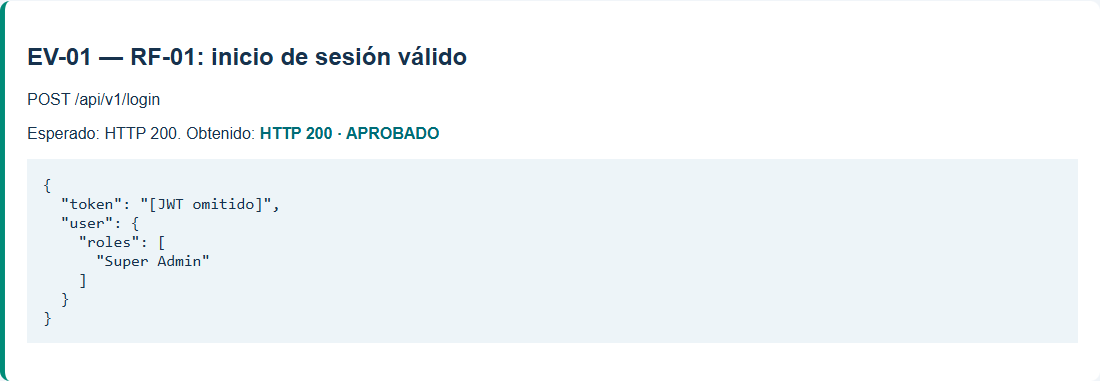
\includegraphics[width=\textwidth]{../../evidencia/http-200.png}
\caption{Inicio de sesión autorizado, CP-01. Fuente: ejecución propia en entorno local.}
\label{fig:prueba-200}
\end{figure}

\begin{figure}[H]
\centering
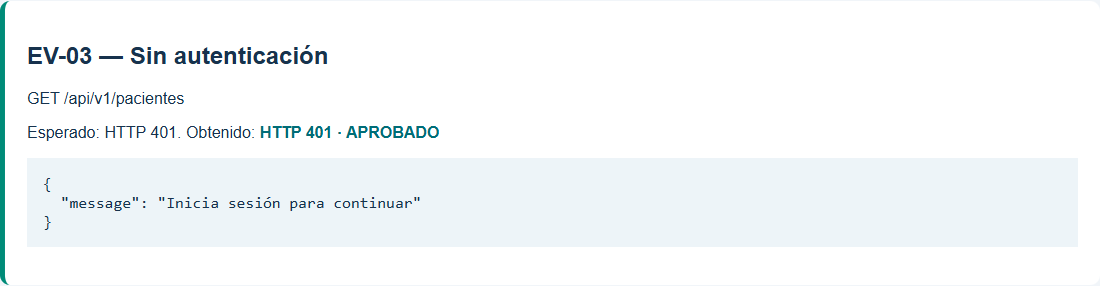
\includegraphics[width=\textwidth]{../../evidencia/http-401.png}
\caption{Acceso a pacientes sin JWT, CP-03. Fuente: ejecución propia en entorno local.}
\label{fig:prueba-401}
\end{figure}

\begin{figure}[H]
\centering
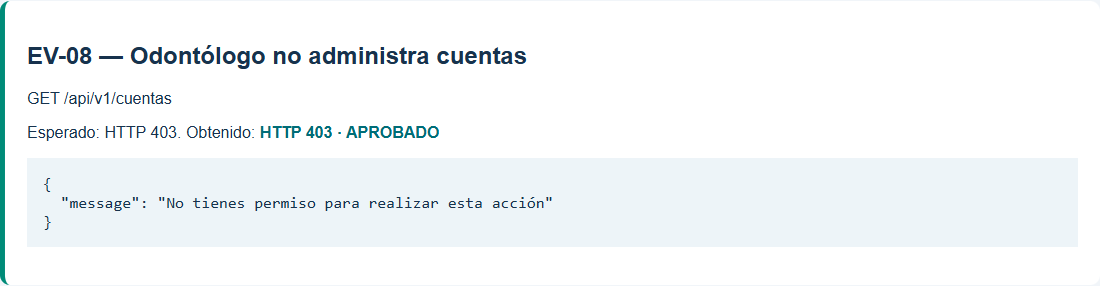
\includegraphics[width=\textwidth]{../../evidencia/http-403.png}
\caption{Consulta de cuentas por un odontólogo, CP-04. Fuente: ejecución propia en entorno local.}
\label{fig:prueba-403}
\end{figure}

\begin{figure}[H]
\centering
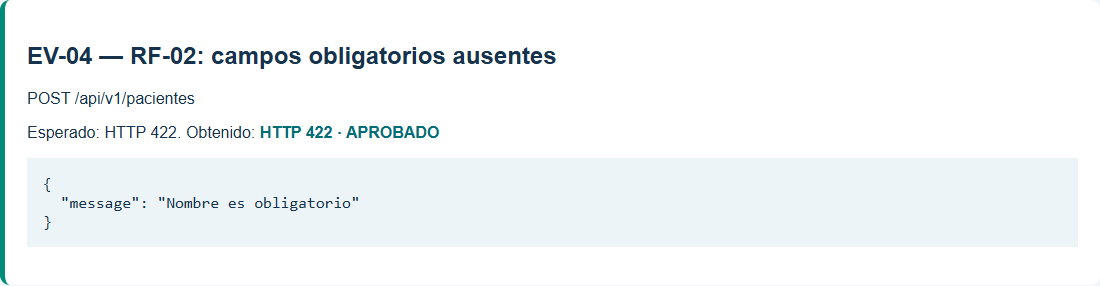
\includegraphics[width=\textwidth]{../../evidencia/http-422.png}
\caption{Registro de paciente sin campos obligatorios, CP-05. Fuente: ejecución propia en entorno local.}
\label{fig:prueba-422}
\end{figure}

El informe ampliado \path{evidencia/evidencias-seguridad.pdf} contiene las
15 respuestas del recorrido de navegador, incluidas la creación de la
solicitud, la generación del enlace y el rechazo del enlace revocado.

\subsection{Comprobaciones en producción y rendimiento}

En el despliegue de Vercel se realizaron comprobaciones de lectura:
la salud de la API respondió 200, el acceso a pacientes sin autenticación
respondió 401, el inicio de sesión respondió 200 y la consulta de solicitudes
radiográficas respondió 200. El detalle se conserva en
\path{evidencia/verificacion-despliegue.json}.

Se midieron diez consultas consecutivas autenticadas al listado de pacientes,
con página de quince registros y sin transferencias de archivos. La medición
incluye el tiempo observado por el cliente HTTP desde este equipo, la red y
la lectura de la respuesta JSON. No es una prueba de concurrencia ni de carga.

\begin{table}[H]\centering
\caption{Tiempos observados en consultas de pacientes en Vercel}
\begin{tabular}{rrr}\toprule
\textbf{Consulta}&\textbf{Estado HTTP}&\textbf{Tiempo (ms)}\\\midrule
1&200&349\\
2&200&214\\
3&200&209\\
4&200&251\\
5&200&219\\
6&200&222\\
7&200&208\\
8&200&320\\
9&200&213\\
10&200&217\\
\bottomrule\end{tabular}\end{table}
En esta muestra, 10 de 10 consultas respondieron en menos de tres
segundos, con un rango de 208 a 349 ms.
Se satisface el umbral de RNF-01 para esta operación y estas condiciones;
el resultado no se generaliza a todas las operaciones ni a usuarios concurrentes.

Las modificaciones de autorización y las nuevas rutas v1 documentadas en esta
revisión se verificaron localmente. El recorrido completo de creación,
enlace y entrega directa a Supabase Storage no se ejecutó en producción
durante esta revisión; las comprobaciones de lectura anteriores no lo
sustituyen. Antes de presentar la versión desplegada debe verificarse ese
recorrido sobre la misma revisión del código.

\section{Despliegue}

El sistema dispone de un entorno accesible mediante Internet, permitiendo
comprobar su funcionamiento fuera del equipo utilizado durante el
desarrollo.

La aplicación se encuentra publicada mediante Vercel y utiliza servicios
externos para la persistencia de información.

La dirección pública del sistema es:

\begin{center}
	
	\url{
		https://proyecto-diplomado-angular-frontend.vercel.app
	}
	
\end{center}

La ruta utilizada para verificar la disponibilidad de la API es:

\begin{center}
	
	\url{
		https://proyecto-diplomado-angular-frontend.vercel.app/api/v1/salud
	}
	
\end{center}

El código fuente se encuentra disponible en:

\begin{center}
	
	\url{
		https://github.com/AdrianLLanos/proyecto-diplomado-angular
	}
	
\end{center}

La configuración de producción utiliza variables de entorno para evitar
incluir credenciales y claves privadas directamente en el repositorio.


% ------------------------------------------------------------
% MONITOREO
% ------------------------------------------------------------

\subsection{Monitoreo de disponibilidad}

La ruta de salud de la API permite verificar si el servicio principal se
encuentra disponible.

Para la entrega final debe mantenerse un servicio de monitoreo que consulte
periódicamente esta ruta y registre el estado de disponibilidad.

% TODO OBLIGATORIO E4:
%
% Servicio utilizado: __________________
% URL pública del monitor: __________________
%
% IMAGEN:
% figuras/monitoreo.png


% ####################################################################
% CAPÍTULO 3
% ####################################################################

\chapter{CONCLUSIONES Y RECOMENDACIONES}


% ============================================================
% 3.1 CONCLUSIONES
% ============================================================

\section{Conclusiones}

Las conclusiones se presentan siguiendo los objetivos específicos definidos
en el Capítulo 1.

\begin{enumerate}
	
	\item
	Respecto al análisis de requisitos, se identificaron los actores, funciones
	principales y características de calidad necesarias para delimitar el
	comportamiento esperado del sistema. La evidencia se presenta en el
	apartado de análisis de requisitos mediante requisitos funcionales, no
	funcionales y casos de uso.
	
	\item
	En relación con el diseño de la solución, se definió una arquitectura
	cliente--servidor que separa la interfaz, la lógica del backend y la
	persistencia de información. También se documentaron las entidades
	principales y la organización general de los módulos.
	
	\item
	Respecto a la implementación, se desarrollaron las funcionalidades que se
	encuentran efectivamente disponibles en la versión final del sistema.
	
	% TODO:
	% Reemplazar la frase anterior por los módulos REALMENTE terminados:
	% autenticación, pacientes, citas, solicitudes, radiografías, etc.
	
	\item
	En relación con la seguridad, el sistema incorpora autenticación y controles
	de autorización para restringir el acceso a las operaciones protegidas.
	Las pruebas realizadas permiten observar respuestas diferentes ante
	usuarios no autenticados y operaciones sin permisos suficientes.
	
	\item
	Respecto a la evaluación del sistema, se establecieron casos de prueba
	reproducibles para comprobar autenticación, autorización, validación y las
	funciones principales. Los resultados finales deben mantenerse respaldados
	por las evidencias obtenidas durante la ejecución.
	
	\item
	Finalmente, el sistema dispone de un entorno público y de un repositorio con
	control de versiones. Esto permite verificar el producto fuera del entorno
	local y disponer de la documentación necesaria para su instalación,
	despliegue y uso.
	
\end{enumerate}


% ============================================================
% 3.2 RECOMENDACIONES
% ============================================================

\section{Recomendaciones}

Se recomienda continuar evaluando el sistema durante su utilización en un
entorno real de la Clínica Odontológica San Martín con el propósito de
obtener métricas relacionadas con tiempos de atención, gestión de citas y
flujo de radiografías.

También se recomienda mantener una revisión periódica de roles y permisos,
especialmente cuando se incorporen nuevas funciones administrativas o
clínicas.

Las pruebas automatizadas deben ampliarse conforme se agreguen nuevos
módulos, de manera que los cambios realizados puedan verificarse antes de
ser publicados.

En cuanto al almacenamiento de archivos clínicos, se recomienda mantener
los documentos dentro de servicios persistentes y evitar su exposición
pública permanente.

Finalmente, pueden desarrollarse nuevas funciones dirigidas a mejorar la
interacción del paciente con la clínica una vez que las funciones actuales
se encuentren estabilizadas y evaluadas.


% ####################################################################
% BIBLIOGRAFÍA
% ####################################################################

\clearpage

\printbibliography[
heading=bibintoc,
title={BIBLIOGRAFÍA CONSULTADA}
]


% ####################################################################
% ANEXOS
% ####################################################################

\clearpage
\appendix


% ============================================================
% ANEXO A
% MANUAL DE USUARIO
% ============================================================

\registraranexo{Manual de usuario}

\chapter{MANUAL DE USUARIO}

\section*{Objetivo}

El presente manual describe las operaciones principales disponibles para
los usuarios autorizados del sistema.

\section*{Ingreso al sistema}

El usuario debe acceder a:

\begin{center}
	\url{https://proyecto-diplomado-angular-frontend.vercel.app}
\end{center}

Posteriormente debe ingresar las credenciales proporcionadas para su perfil.

% IMAGEN:
% figuras/manual-login.png


\section*{Gestión de pacientes}

El usuario autorizado puede ingresar al módulo correspondiente para
consultar pacientes y utilizar las operaciones habilitadas según su perfil.

% IMÁGENES:
% figuras/manual-pacientes.png
% figuras/manual-paciente-nuevo.png


\section*{Gestión de citas}

El módulo de citas permite consultar y registrar información relacionada
con la programación de atención.

% IMÁGENES:
% figuras/manual-citas.png


\section*{Gestión de radiografías}

El flujo radiográfico comprende la creación de la solicitud, la generación
del acceso correspondiente, la recepción del archivo y su posterior
consulta.

% IMÁGENES NECESARIAS:
%
% figuras/manual-solicitud-radiografia.png
% figuras/manual-acceso-radiografia.png
% figuras/manual-carga-radiografia.png
% figuras/manual-consulta-radiografia.png


% ============================================================
% ANEXO B
% INSTALACIÓN Y DESPLIEGUE
% ============================================================

\registraranexo{Manual de instalación y despliegue}

\chapter{MANUAL DE INSTALACIÓN Y DESPLIEGUE}

\section*{Requisitos}

Para ejecutar el proyecto en un entorno de desarrollo se requiere contar
con Node.js, npm, acceso a los servicios utilizados por la aplicación y las
variables de entorno correspondientes.

\section*{Clonación}

\begin{verbatim}
	git clone https://github.com/AdrianLLanos/
	proyecto-diplomado-angular.git
	
	cd proyecto-diplomado-angular
\end{verbatim}

\section*{Instalación de dependencias}

\begin{verbatim}
	npm install
\end{verbatim}

\section*{Variables de entorno}

Las credenciales y claves sensibles deben mantenerse mediante variables de
entorno.

No se deben incorporar valores reales de producción dentro del documento
ni dentro del repositorio.

\section*{Ejecución}

Los comandos exactos correspondientes al frontend y backend deben tomarse
del archivo README vigente del repositorio.

\section*{Pruebas}

Las pruebas automatizadas pueden ejecutarse mediante:

\begin{verbatim}
	npm run test:report
\end{verbatim}

\section*{Despliegue}

La versión pública se encuentra desplegada mediante Vercel.

Las variables necesarias para producción se configuran desde la plataforma
de despliegue sin incorporarlas directamente al código.


% ============================================================
% ANEXO C
% REPOSITORIO
% ============================================================

\registraranexo{Repositorio de código}

\chapter{REPOSITORIO DE CÓDIGO}

El código fuente se encuentra disponible en:

\begin{center}
	
	\url{
		https://github.com/AdrianLLanos/proyecto-diplomado-angular
	}
	
\end{center}

El repositorio utiliza Git como sistema de control de versiones y mantiene
el historial correspondiente al desarrollo del proyecto.


% ============================================================
% ANEXO D
% DIRECCIÓN PÚBLICA
% ============================================================

\registraranexo{Dirección pública del sistema}

\chapter{DIRECCIÓN PÚBLICA DEL SISTEMA}

La aplicación web se encuentra disponible en:

\begin{center}
	
	\url{
		https://proyecto-diplomado-angular-frontend.vercel.app
	}
	
\end{center}

La ruta utilizada para comprobar el estado de la API es:

\begin{center}
	
	\url{
		https://proyecto-diplomado-angular-frontend.vercel.app/api/v1/salud
	}
	
\end{center}


% ============================================================
% ANEXO E
% DIAGRAMAS
% ============================================================

\registraranexo{Diagramas}

\chapter{DIAGRAMAS}

En este anexo se incorporan los diagramas cuya dimensión dificulta su
lectura dentro del cuerpo principal del documento.

% INSERTAR:
%
% figuras/casos-uso.png
% figuras/modelo-er.png
% figuras/arquitectura-completa.png
% figuras/flujo-radiografias.png


% ============================================================
% ANEXO F
% EVIDENCIAS
% ============================================================

\registraranexo{Evidencias técnicas}

\chapter{EVIDENCIAS TÉCNICAS}

En este anexo se presentan las evidencias complementarias obtenidas durante
las pruebas y el despliegue del sistema.

\section*{Pruebas automatizadas}

El reporte correspondiente se mantiene en:

\begin{center}
	\texttt{evidencia/reporte-pruebas-e3.txt}
\end{center}

\section*{Despliegue}

% IMÁGENES:
%
% figuras/vercel-despliegue.png
% figuras/api-salud.png

\section*{Monitoreo}

% IMAGEN:
%
% figuras/monitoreo.png

\section*{Rendimiento}

% IMAGEN O TABLA:
%
% evidencia de las mediciones reales del RNF-01.
\end{document}